\documentclass[../../main.tex]{subfiles}
\begin{document}
\graphicspath{{./figures}}
\chapter{Preprocesamiento de los datos adquiridos}\label{cap::preproc}
Las señales externas son muestreadas por el ADC a 65~MSps en un ancho de banda de 25~MHz como se desarrolló en el \cref{sec::planteo-front-end}. Sin embargo, los \textit{beams} de salida poseen un ancho de banda de apenas 25~kHz, de manera que puede reducirse considerablemente tanto el ancho de banda como la tasa de muestreo. Si se lograse centrar el ancho de banda de un  \textit{beam} en banda base por ejemplo, este solo ocuparía $12.5\un{kHz}$. Esto permitiría teóricamente reducir el ancho de banda de trabajo a $12.5\un{kHz}$ y trabajar con una tasa de muestreo ligeramente superior a 25~kSps cumpliendo con el teorema del muestreo~\cite{teorema-del-muestreo} \unsure{JQ: por lo general fs/2 no es suficiente para procesar. Lo importante acá es que bajás órdenes de magnitud en el ancho de banda. Capaz refrasearía diciendo que el ancho de banda final debería ajustarse en función de los reqs de performance del sistema}.

Como se dijo en el \cref{sec::planteo-sist-adq}, esta parte del \textit{core} de adquisición se desarrolla en el presente proyecto. Su diseño, implementación y validación se realizaron primero de manera aislada e independiente a lo desarrollado en~\cite{proyecto-jose} y, posteriormente, se integró dentro de dicho sistema.

\section{Requerimientos de diseño}
La etapa de preprocesamiento debe ser capaz de seleccionar uno o varios canales de frecuencia de 25~kHz de ancho de banda, a partir de ahora a estos se les llamará \textit{beams} o haces, reservándose el término \textit{canal} para los canales del ADC.

Luego, partiendo de la banda de UHF de 3~MHz de ancho de banda centrada en $18.5\un{MHz}$ tras el submuestreo, debe obtenerse a la salida uno o varios haces de 25~kHz de ancho de banda.

\section{Diseño conceptual}\label{sec::disenio-conceptual-preproc}
Se parte de la señal real ya submuestreada cuyo espectro está cetrado en $\pm 18.5\un{MHz}$ (ver figura \ref{fig::undersampling}) y su módulo  es simétrico respecto a la frecuencia $f = 0$, como se ilustra en la figura \ref{fig::espectro-inicial}. Dentro de cada triángulo en dicho gráfico se encuentran todos los haces de 25~kHz, replicados a ambos lados del espectro. Esto implica una redundancia de información que puede aprovecharse para optimizar la etapa de preprocesamiento.

Se propone entonces trabajar sobre solo una de estas réplicas mediante una mezcla compleja, esto es, una rotación del espectro que permita llevar una de las copias mostradas en \ref{fig::espectro-inicial} a banda base. En este caso es indistinto cuál de las copias se selecciona. 

Asumiendo AWGN, se tiene en el espectro una densidad de potencia de ruido independiente de la frecuencia. Tras el corrimiento de una de las réplicas a BB se procede a realizar también un filtrado como se muestra en la figura \ref{fig::espectro-banda-corrida} reduciendo el ancho de banda de trabajo de manera de filtrar gran parte del ruido entrante. Esta es una primera etapa de ganancia de preprocesamiento, la cual se analizó en el \cref{sec::ganancias-por-preproc}. 

Como puede verse en la figura \ref{fig::espectro-banda-corrida} el ancho de banda del filtro debe ser ligeramente superior a $1.5\un{MHz}$ de manera de tolerar el corrimiento Doppler producido durante la pasada del satélite, el cual puede alcanzar corrimientos de hasta $\pm 10\un{kHz}$, como se desarrolla en el apéndice \ref{ap::doppler}.

Una vez aislada una copia de la banda de interés, resta seleccionar el \textit{beam} que quiere recibirse. Esto puede hacerse mediante un procedimiento similiar al recién aplicado. En este caso, la señal es compleja ya que no hay simetría en el módulo del espectro respecto a $f = 0$, es decir que no existe la redundancia de información que existía al hacer la primer mezcla. Esto implica que el sentido en el que se rota el espectro es relevante.

En la figura \ref{fig::espectro-canal} se muestra el módulo del espectro tras realizar una segunda mezcla compleja partiendo de lo mostrado en la figura \ref{fig::espectro-banda-corrida} para trasladar a BB al haz de interés. El rectángulo en línea de puntos que se muestra en dicha figura representa el filtrado que debe aplicarse tras la mezcla, el cual atenuará el resto de la banda junto con la parte de la potencia de ruido que cae por fuera de la banda de interés, obteniéndose así una segunda ganancia de preprocesamiento.

Nuevamente, si bien los haces tienen 25~kHz de ancho de banda, el filtrado debe contemplar un margen para tolerar el corrimiento Doppler (ver apéndice \ref{ap::doppler}).

\figura[0.8]{espectro-inicial}{Ilustración del módulo del espectro a la entrada de la etapa del preprocesamiento. Se tiene la banda de interés sobre un piso de AWGN. Se ve que el espectro es simétrico respecto a la frecuencia $f = 0$ ya que se trata de una señal real.}

\figura[0.8]{espectro-banda-corrida}{Módulo del espectro de la banda de interés trasladada a banda base y filtrada.}

\figura[0.8]{espectro-canal}{Módulo del espectro de la banda de interés centrada en el haz de interés tras la segunda mezcla compleja. El rectángulo en línea punteada representa el filtrado que debe aplicarse psoteriormente para atenuar el resto de la banda y el ruido que cae por fuera del ancho de banda del haz de interés.}

\section{Prueba de concepto en software}
A modo de primera comprobación del diseño conceptual previo a su implementación en hardware, se hizo una prueba de concepto en software de la etapa de preprocesamiento empleando Python. 
Esta se encuentra en \texttt{Simulaciones/preprocesamiento.ipynb}. 

Partiendo de la señal submuestreada a 65~MSps mostrada en la figura \ref{fig::undersampling} se aplicó un DDC~\cite{DDC}, cuyo diagrama de bloques se muestra en la figura \ref{fig::DDC}. 
Este incluye un NCO el cual genera una exponencial compleja para realizar la rotación de espectro en sentido horario a una frecuencia de $18.5\un{MHz}$, de manera de trasladar la banda de $[-20\un{MHz}, -17\un{MHz}]$ a $[-1.5\un{MHz}, 1.5\un{MHz}]$. 

Ya en banda base, el DDC contiene una etapa de filtrado pasabajos, cuya frecuencia de corte se configuró como $f_c = 1.5\un{MHz}$ de manera de capturar toda la banda de interés dentro de la banda de paso del filtro. El filtrado aplicado fue de tipo Butterworth~\cite{Butterworth} y sus coeficientes del mismo se obtuvieron mediante la función \texttt{butter}~\cite{butter} de la librería de SciPy~\cite{scipy} y el filtrado propiamente dicho se realizó usando la función \texttt{lfilter}~\cite{lfilter} también de la librería de SciPy. 

Por último, el DDC posee una etapa de decimación en la cual se reduce la tasa de muestreo. Para determinar el factor de decimación debe tenerse en cuenta que la tasa de Nyquist~\cite{Nyquist-rate} es ahora de 3~MHz, lo cual implica que la tasa actual de muestreo de 65~MSps podría reducirse hasta en un factor $65/3 = 21.66$ aproximadamente. 
No obstante, para esta prueba de concepto se eligió un factor de decimación de 10, de manera que la tasa de muestras a la salida del DDC resulta $6.5\un{MSps}$. La salida de este primer DDC se muestra en la figura \ref{fig::DDC-band}.

Teniendo toda la banda de UHF ya en BB, se procede a seleccionar un haz o \textit{beam} como se muestra en la figura \ref{fig::espectro-canal}. 
Para esto se instancia un nuevo DDC, el cual realiza la mezcla compleja para trasladar el haz a banda base, ejecuta un filtrado del haz con una frecuencia de corte de $f_c = 12.5\un{kHz}$\footnote{Al tratarse de una prueba de concepto, no se tuvo en cuenta el corrimiento Doppler. 
De tenerse en cuenta, debería aumentarse la frecuencia de corte del filtro aproximadamente 10~kHz por encima de la actual.} y finalmente una decimación. 
Para esta última se empleo un factor de decimación igual a 100. La salida de este segundo DDC se muestra en la figura \ref{fig::DDC-beam}, donde se observa que pudo aislarse un haz de 25~kHz de ancho de banda de manera exitosa.

\figura[0.7]{DDC}{Diagrama de bloques de un \textit{Digital Down Converter} (DDC).}

\begin{figure}[H]
    \centering
    \subcaptionbox{Salida del primer DDC encargado de trasladar la banda de interés a BB, filtrar y luego decimar con un factor 10.\label{fig::DDC-band}}
    {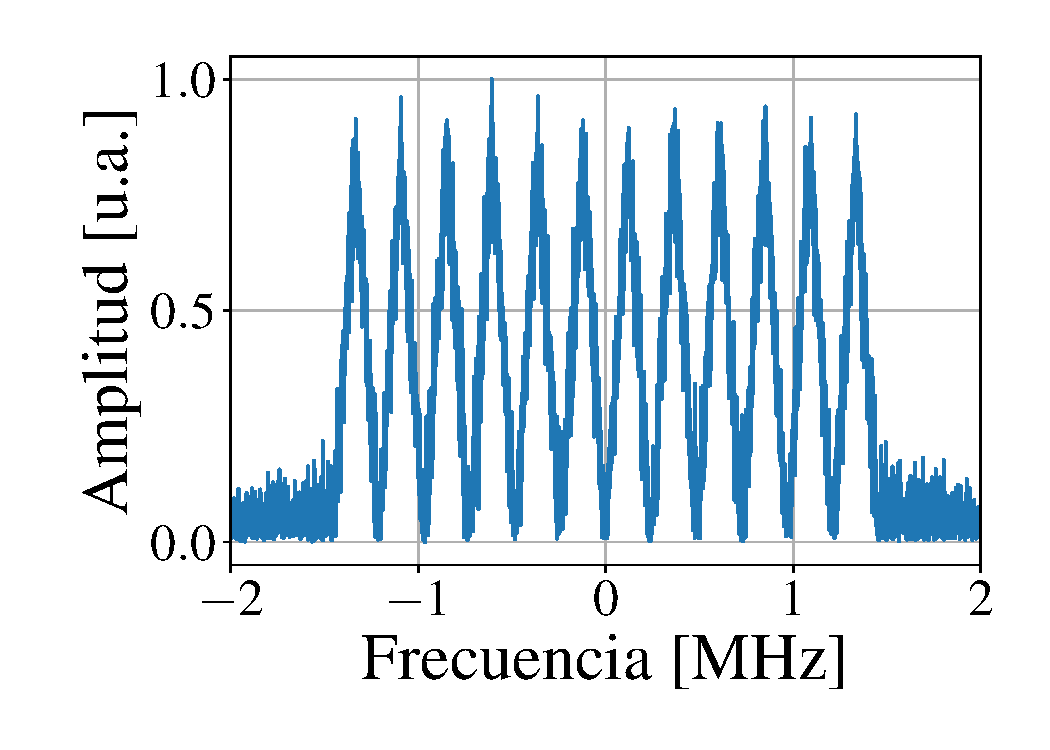
\includegraphics[width=0.49\linewidth]{DDC-band.pdf}}
    \hspace{\fill}%\\[1PC]
    \subcaptionbox{Salida del segundo DDC encargado de seleccionar un \textit{beam}, trasladarlo a BB, filtrarlo y reducir la tasa de muestreo. Se dibuja además una línea vertical en la frecuencia donde termina el canal de interés, esto es, $f = 12.5\un{kHz}$.\label{fig::DDC-beam}}
    {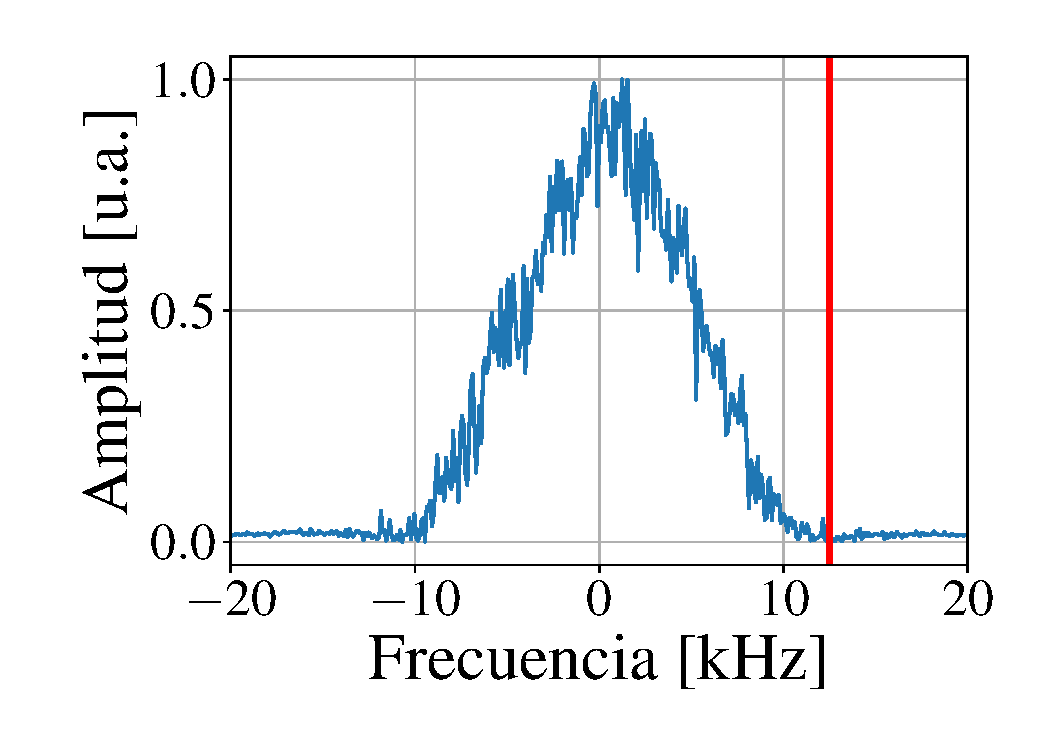
\includegraphics[width=0.49\linewidth]{DDC-beam.pdf}}
    \caption{Salida de las dos etapas de DDCs.}
    \label{fig::DDC-output}
\end{figure}

\section{Implementación en hardware}
Habiendo validado el diseño conceptual mediante una implementación en software se procede a realizar una implementación del mismo en la placa CIAA-ACC. Dado que el SoC Zynq-7030 incluido en la CIAA-ACC es fabricado por la compañía Xilinx, se hizo uso de su entorno de desarrollo, el cual incluye al software \textit{Vivado}~\cite{vivado} para el desarrollo, síntesiss e implementación en la FPGA y al software \textit{Vitis Unified Software Platform}~\cite{vitis} para el desarrollo y la compilación cruzada~\cite{cross-compilation} del software para el PS. La versión del entorno de desarrollo usada en este proyecto fue la 2020.2.

La tasa de muestreo del AD9249 es de 65~MSps como se indica en la tabla \ref{tab::ADC}, esto fija la tasa de datos que tiene que procesar la FPGA y representa una frecuencia mínima de reloj a emplear. En base a esto, se eligió una frecuencia de reloj de 260~MHz para realizar el preprocesamiento de manera de disponer de 4 ciclos de reloj entre cada muestra que entrega el ADC\footnote{$260\un{MHz} = 4 \cdot 65\un{MHz}.$}. Esto puede otorgar cierta flexibilidad a la hora de diseñar el \textit{pipeline} de preprocesamiento.

Esta implementación es de tipo \textit{standalone}, es decir, se hizo de manera aislada al sistema desarrollado en~\cite{proyecto-jose} y se consideró un único \textit{beam} de salida como primera prueba de concepto.

Un esquema general con finalidad de servir como guía para la implementación se muestra en la figura \ref{fig::disenio-para-hw}, donde las señales de datos se encuentran en negro y las de control en naranja. En esta figura también se observan las etapas de mezcla y filtrado concebidas en la sección \ref{sec::disenio-conceptual-preproc} junto con los bloques
\begin{itemize}
    \item \texttt{Data source hier}: su objetivo es controlar la fuente de datos que ingresa al preprocesamiento, sobre todo con finalidades de \textit{debug} como se explicará en breve en la subsección \ref{subsec::debug-preproc-inicial}.
    \item \texttt{AXI hier}: este bloque agrupa todo el hardware relacionado a la interconexión con el PS lo cual permitirá controlar la \texttt{Data source hier} mediante registros.
\end{itemize}

\figura[0.85]{disenio-para-hw}{Esquema guía para la implementación de la etapa de preprocesamiento en hardware. Se indican en negro las señales de datos y en naraja las de control.}

\subsection{IPs empleadas}
\textit{Vivado} cuenta con interfaces o bloques propietarios en su librería de propiedad intelectual o IP~\cite{IP-Xilinx}. Estos \textit{IP Blocks}, a partir de ahora simplemente IPs, funcionan como caja negra para el usuario ya que su implementación está encriptada. Los IPs actuan recibiendo entradas y produciendo salidas acordes a su funcionalidad.

En el desarrollo de la etapa de preprocesamiento se utilizaron las IPs de \textit{Vivado} nombradas en la tabla \ref{tab::ip-vivado-preproc}.
\begin{table}[H]
    \centering
    \resizebox{\textwidth}{!}{%
    \begin{tabular}{|llc|}
    \hline
    \multicolumn{3}{|c|}{\textbf{IPs nativas utilizadas}}                                                                                                                                                                                                                                                        \\ \hline
    \multicolumn{1}{|l|}{\textbf{Nombre}}    & \multicolumn{1}{l|}{\textbf{Función}}                                                                                                                                                                                  & \textbf{Documentación}                   \\ \hline
    \multicolumn{1}{|l|}{\texttt{AXI Interconnect}}   & \multicolumn{1}{l|}{\begin{tabular}[c]{@{}l@{}}Conecta uno o más dispositivos maestros AXI mapeados\\ en memoria a uno o más dispositivos esclavos mapeados\\ en memoria.\end{tabular}}                                &~\cite{axi-interconnect} \\ \hline
    \multicolumn{1}{|l|}{\texttt{Complex Multiplier}} & \multicolumn{1}{l|}{\begin{tabular}[c]{@{}l@{}}Implementa multiplicadores complejos optimizados, de\\ alto rendimiento y compatibles con AXI4-Stream basados\\ en opciones especificadas por el usuario.\end{tabular}} &~\cite{complex-mult}     \\ \hline
    \multicolumn{1}{|l|}{\texttt{DDS Compiler}}       & \multicolumn{1}{l|}{Genera señales sinusoidales.}                                                                                                                                                                      &~\cite{dds-compiler}     \\ \hline
    \multicolumn{1}{|l|}{\texttt{FIR Compiler}}       & \multicolumn{1}{l|}{Genera un filtro tipo FIR.}                                                                                                                                                                        &~\cite{fir-compiler}     \\ \hline
    \end{tabular}%
    }
    \caption{IPs nativas utilizadas en el desarrollo de la etapa de preprocesamiento.}
    \label{tab::ip-vivado-preproc}
    \end{table}

\subsection{Módulos desarrollados}
Además de emplear IPs de \textit{Vivado}, se desarrollaron módulos en VHDL accesibles en el directorio \texttt{Fpga/prj/preprocessing\_stage/src}. Dichos módulos y su función se mencionan a continuación en la tabla \ref{tab::ip-fran}.

La integración de estos módulos con las IPs de Xilinx serán más claras en breve cuando se explique la composición del sistema implementado.

\begin{table}[H]
\centering
    \resizebox{0.9\textwidth}{!}{%
    \begin{tabular}{|ll|}
    \hline
    \multicolumn{2}{|c|}{\textbf{Módulos desarrollados para preprocesamiento}}                                                                                                                                                                                                                                                                                                                                                               \\ \hline
    \multicolumn{1}{|l|}{\textbf{Nombre}}                                                   & \textbf{Función}                                                                                                                                                                                                                                                                                                         \\ \hline
    \multicolumn{1}{|l|}{\texttt{AXI Slave Reg}}                                                     & Bloque de registros que implementan el protocolo AXI4-Lite.                                                                                                                                                                                                                                                              \\ \hline
    \multicolumn{1}{|l|}{\texttt{Basic Counter}}                                                     & \begin{tabular}[c]{@{}l@{}}Contador de ancho ajustable que se incrementa cada N \\ ciclos de reloj, con N configurable.\end{tabular}                                                                                                                                                                                     \\ \hline
    \multicolumn{1}{|l|}{\texttt{CDC Comparator}}                                                    & Compara dos entradas y la asigna a la salida en caso de ser iguales.                                                                                                                                                                                                                                                     \\ \hline
    \multicolumn{1}{|l|}{\texttt{CDC Two FF Sync}}                                                   & \begin{tabular}[c]{@{}l@{}}Dos FF en serie. Sirven para sincronizar un bit de una señal\\ asíncrona.\end{tabular}                                                                                                                                                                                                        \\ \hline
    \multicolumn{1}{|l|}{\texttt{Complex Gain}}                                                      & Ganancia de 6 dB para una señal de entrada compleja.                                                                                                                                                                                                                                                                     \\ \hline
    \multicolumn{1}{|l|}{\texttt{Data Source Mux}}                                                   & \begin{tabular}[c]{@{}l@{}}Multiplexor con 3 entradas tipo AXI4-Stream y una señal\\ de control.\end{tabular}                                                                                                                                                                                                            \\ \hline
    \multicolumn{1}{|l|}{\begin{tabular}[c]{@{}l@{}}\texttt{DDS Compiler}\\ \texttt{Controller}\end{tabular}} & \begin{tabular}[c]{@{}l@{}}Opera con la interfaz AXI4-Stream. Su entrada es la salida de\\ un \texttt{DDS Compiler}. Mediante el pulso de tready del protocolo\\ AXI4-Stream controla la tasa a la cual el \texttt{DDS Compiler} \\ genera nuevos datos, convirtiendola en cualquier submúltiplo de\\ la frecuencia de reloj.\end{tabular} \\ \hline
    \multicolumn{1}{|l|}{\begin{tabular}[c]{@{}l@{}}\texttt{Valid Data}\\ \texttt{Holder}\end{tabular}}       & \begin{tabular}[c]{@{}l@{}}Opera con la interfaz AXI4-Stream. Sostiene el último dato\\ válido en la salida hasta que llega uno nuevo.\end{tabular}                                                                                                                                                                      \\ \hline
    \multicolumn{1}{|l|}{\texttt{Zero Padder}}                                                       & \begin{tabular}[c]{@{}l@{}}Convierte una señal de N bits en una de M bits con M\textgreater{}N\\ agregando ceros ya sea a derecha o a izquierda.\end{tabular}                                                                                                                                                            \\ \hline
    \end{tabular}%
    }
    \caption{Módulos desarrollados en VHDL para el desarrollo de la etapa de preprocesamiento.}
    \label{tab::ip-fran}
    \end{table}

\subsection{Filtros y decimación}\label{subsec::filtros-decimacion}
Según el esquema guía de la figura \ref{fig::disenio-para-hw} y lo desarrollado en \ref{sec::disenio-conceptual-preproc} deben implementarse dos etapas digitales de filtrado pasabajos y decimación, una después de realizar cada mezcla. 

Al diseñar la etapa de filtrado deben tenerse en cuenta las consideraciones habituales como la evaluación del tipo de filtro, la frecuencia de corte, el orden del filtro, entre otros. Pero además, al tratarse de un filtro a ser implementado en hardware, debe tenerse en cuenta que el mismo hará uso de aritmética de punto fijo~\cite{pto-fijo}. Esto implica que el número de dígitos decimales con los que se trabaja se mantiene constante.

\subsubsection{Diseño de los filtros}
Para el diseño de los filtros se utilizó el programa MATLAB de la empresa MathWorks, el cual incorpora herramientas tales como \texttt{Filter Builder}~\cite{filter-builder} y \texttt{Filter Designer}~\cite{filter-designer}. Estas herramientas permiten realizar el diseño de filtros de todo tipo a partir de los parámetros de interés de cada aplicación en particular. 

\texttt{Filter Builder} y \texttt{Filter Designer} también son capaces de trabajar con aritmética de punto fijo y generar el código en VHDL para utilizar directamente en \textit{Vivado}. A priori esta puede ser una opción viable, sin embargo, dado que los filtros se implementarán con el \textit{IP Block} \texttt{FIR Compiler} nativo de Xilinx, no se necesita el código en VHDL. En cambio, el \texttt{FIR Compiler} requiere que se lo configure con los valores de los coeficientes. Para esto se usa un archivo con extensión \textit{coe} que es un archivo de texto indicando los valores de todos los coeficientes, la base numérica en la que están expresados (llamado \textit{radix}) y el ancho en bits de los mismos. Un recorte de un archivo de coeficientes se muestra en la figura \ref{fig::coef-file}. Este recorte corresponde al archivo empleado en la configuración del primer filtro pasabajos.

Resulta relevante destacar que finalmente, a pesar de las capacidades de operación con aritmética de punto fijo que tienen las herramientas de MATLAB, el diseño de los filtros se hizo con aritmética de punto flotante. La razón detrás de esto es que \textit{Vivado}, a través del \texttt{FIR Compiler}, cuenta con su propio método de implementación en punto fijo a partir de punto flotante. Es decir, el \texttt{FIR Compiler} puede configurarse con aritmética de punto flotante y él mismo se encarga de convertirlo a aritmética de punto fijo.

El primer filtrado se designará a partir de ahora como \textit{filtrado de banda}. Este nombre proviene del hecho de que este es el filtrado a ser aplicado tras la traslación de la banda de interés a BB. Este filtrado debe contener a la banda de interés en su banda de paso. Al estar en BB, la máxima frecuencia de la banda de interés de 3~MHz de ancho de banda es $f_\textrm{max} = 1.5\un{MHz}$. Luego, usando la herramienta \texttt{Filter Designer} se generaron los coeficientes para un filtro FIR pasabajos de tipo equirripple. La respuesta del mismo junto con sus configuraciones se muestran en la figura \ref{fig::band-filter.png}. Además, sus especificaciones se listan en la tabla \ref{tab::filtros-preproc}.

Para el caso del segundo filtrado, a partir de ahora \textit{filtrado de haz} o \textit{filtrado de beam}, se opera de forma análoga al anterior. En este caso se tiene el requerimiento de que cada beam tiene alrededor de 25~kHz de ancho de banda en total. Al estar en BB, la frecuencia más alta es de la mitad del ancho de banda ($12.5\un{kHz}$), sin embargo, debe incorporarse un margen para contemplar el corrimiento Doppler (ver apéndice \ref{ap::doppler}). Como una primera iteración se diseñó un filtro de 50~kHz de ancho de banda, cuyas especificaciones se encuentran en la tabla \ref{tab::filtros-preproc} y su respuesta en frecuencia se ilustra en la figura \ref{fig::beam-filter-old}.

\figura[0.7]{coef-file}{Ejemplo de archivo de configuración generado con MATLAB para el \texttt{FIR Compiler}.}

\subsubsection{Tasas de decimación}
Tras el primer filtrado se tiene toda la información de la banda de UHF de interés ahora en el rango de frecuencias $-1.5\un{MHz}<f<1.5\un{MHz}$. De esta manera, se requiere una tasa de muestreo mínima superior a los 3~MHz (\cite{teorema-del-muestreo}). Partiendo de la tasa actual de muestreo de 65~MSps, puede incorporarse un factor de decimación máximo:
\[\textrm{Factor de decimación máximo} = \left\lfloor\frac{65\un{MSps}}{3\un{MSps}}\right\rfloor = 21.\]
Para esta implementación \textit{standalone} se eligió un factor de decimación de 8. Este parámetro es configurable directamente en el \texttt{FIR Compiler}, el cual se encarga de la optimización de recursos~\cite{fir-compiler}. Así, la tasa de datos a la salida del filtrado de banda es $f'_s = 8.125\un{MHz}$.

Tras el filtrado de canal se tiene que a la salida el ancho de banda es de 50~kHz. Luego, se requiere una frecuencia de muestreo de al menos 100~kHz. Esto permite tener el siguiente factor máximo de decimación:
\[\textrm{Factor de decimación máximo} = \left\lfloor\frac{8.125\un{MSps}}{100\un{kSps}}\right\rfloor = 81.\] En este caso se eligió una tasa de decimación de 50.

\begin{table}[H]
    \centering
    \resizebox{0.7\textwidth}{!}{%
    \begin{tabular}{|l|c|c|}
    \hline
    \multicolumn{1}{|c|}{}                  & Filtro de banda & Filtro de haz \\ \hline
    Frecuencia de paso {[}kHz{]}            & 1500            & 50          \\ \hline
    Frecuencia de rechazo {[}kHz{]}         & 2000              & 100           \\ \hline
    Atenuación en banda de paso {[}dB{]}    & 0               & 0             \\ \hline
    Atenuación en banda de rechazo {[}dB{]} & 40              & 40            \\ \hline
    Tipo de filtro                          & Equirriple      & Equirriple    \\ \hline
    Orden del filtro                        & 185             & 231           \\ \hline
    Frecuencia de muestreo {[}Msps{]}       & 65              & 8,125         \\ \hline
    Factor de decimación                    & 8               & 50            \\ \hline
    \end{tabular}%
    }
    \caption{Configuraciones principales de los filtros de banda y de haz.}
    \label{tab::filtros-preproc}
\end{table}

\begin{figure}[H]
    \centering
    \subcaptionbox{Diseño del filtro de banda.\label{fig::band-filter.png}}
    {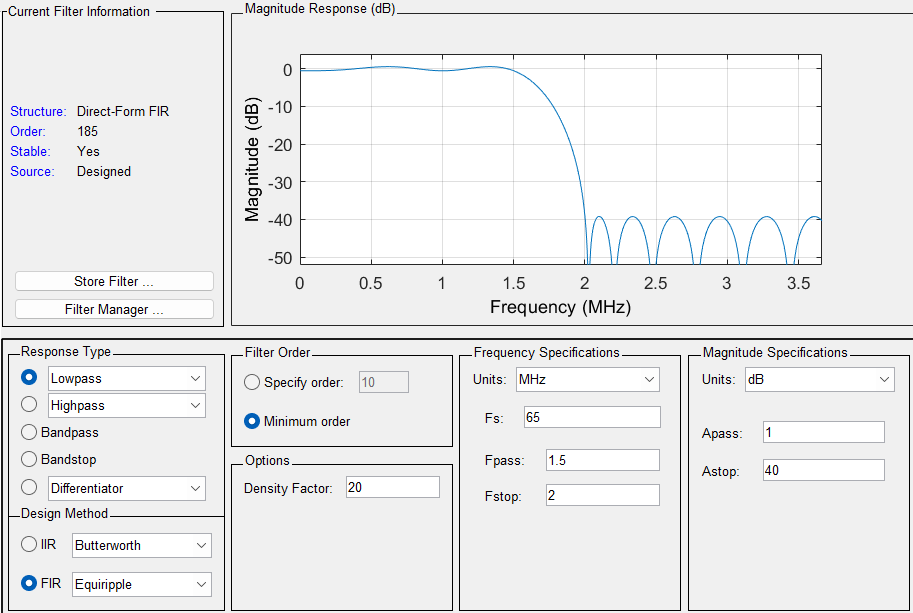
\includegraphics[width=0.7\linewidth]{band-filter.png}}
    \\[1PC]
    \subcaptionbox{Diseño del filtro de haz\label{fig::beam-filter-old.png}}
    {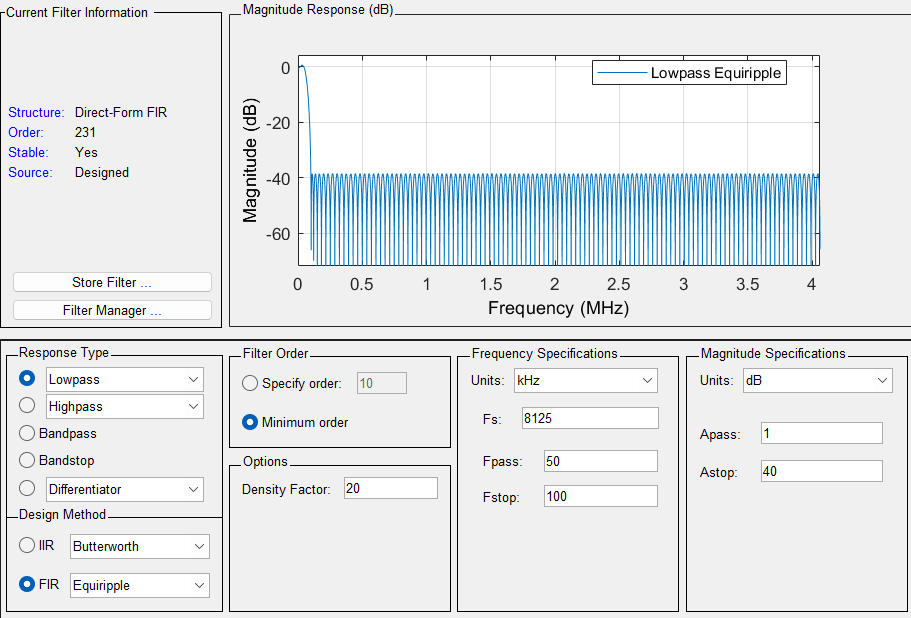
\includegraphics[width=0.7\linewidth]{beam-filter-old.png}}
    \caption{Diseño de filtros empleando la herramienta \texttt{Filter Designer}.}
    \label{fig::filter-designs-old}
\end{figure}

\subsection{Herramientas de \textit{debug}}\label{subsec::debug-preproc-inicial}
En todo desarrollo resulta importante incorporar herramientas para poder \textit{debuggear} el sistema cuando algo no esté funcionando. Con este propósito se empleó el módulo \texttt{Data Source Mux} mencionado en la tabla \ref{tab::ip-fran} al cual se conectaron tres entradas:
\begin{itemize}
    \item Los datos del ADC. Este es el modo de operación normal, no de \textit{debug}.
    \item Una instancia del módulo \texttt{Basic Counter} (ver tabla \ref{tab::ip-fran}).
    \item Una instancia del IP \texttt{DDS Compiler} oscilando a una frecuencia conocida y controlado mediante una instancia de \texttt{DDS Compiler Controller} (ver tablas \ref{tab::ip-vivado-preproc} y \ref{tab::ip-fran}).
\end{itemize}

El multiplexor se controla mediante un registro en el módulo \texttt{AXI Slave Reg} conectado a su vez al IP \texttt{AXI Interconnect}. Los valores que puede asumir la señal de control y la correspondiente salida asignada se especifican en la tabla \ref{tab::data-source-mux}.

\begin{table}[H]
\centering
\begin{tabular}{|ll|}
\hline
\multicolumn{2}{|c|}{$\texttt{Data Source Mux}$} \\ \hline
\multicolumn{1}{|l|}{\textbf{Valor}} & \textbf{Selección} \\ \hline
\multicolumn{1}{|l|}{0} & Datos del ADC \\ \hline
\multicolumn{1}{|l|}{1} & Oscilador local de $\textit{debug}$ \\ \hline
\multicolumn{1}{|l|}{2} & Contador de $\textit{debug}$ \\ \hline
\end{tabular}
\caption{Selección de la señal de salida del multiplexor de fuente de datos en según el valor que toma la señal de control.}\label{tab::data-source-mux}
\end{table}

\subsection{Cruces de dominio de reloj (CDCs)}\label{subsec::cdcs-standalone}
Un dominio de reloj se compone de todos los elementos de un circuito lógico que operan bajo la misma señal de \textit{clock}.

Al realizar desarrollo en hardware, una situación que se presenta con regularidad es la necesidad de sincronizar con un dado reloj una señal que proviene de otro dominio de reloj. Esta situación recibe el nombre de \textit{Clock Domain Crossing} (CDC) y debe ser manejada de manera de poder asegurar el cumplimiento de los tiempos de \textit{setup} y \textit{hold} de los \textit{flip-flops} controlados por el nuevo reloj.

En el caso de la señal de control del \texttt{Data Source Mux}, la misma se encuentra dentro del dominio de reloj del \texttt{AXI Interconnect} (el cual generalmente viene dado por el PS). Al tratarse de una señal lenta ya que cambia en tiempos muy largos, puede sincronizarse en el nuevo dominio de reloj (esto es, el de 260~MHz) como si se tratara de una señal asíncrona. Para esto se hace uso del módulo \texttt{CDC Two FF Sync}.

Sin embargo, dicho módulo por si solo se emplea para sincronizar un único bit. En este caso, la señal de control del multiplexor tiene 2 bits (hay 3 entradas), en consecuencia, para asegurar la integridad de la señal en el CDC se emplean dos \texttt{CDC Two FF Sync} en serie y se comparan sus salidas con el módulo \texttt{CDC Comparator} como se muestra en la figura \ref{fig::CDC-preproc}. Si ambas salidas son iguales, entonces la señal se sincroniza exitosamente al dominio de reloj de 260~MHz.

\figura{CDC-preproc}{Sincronizador de 2 bits para señales lentas empleado para realizar el CDC de la señal de control del multiplexor desde el dominio de reloj del \texttt{AXI Interconnect} al dominio de reloj de 260~MHz.}

\subsection{Implementación en \textit{Vivado}}\label{subsec::implementacion-vivado}
Haciendo uso e interconectando los bloques de IP de las tablas \ref{tab::ip-vivado-preproc} y \ref{tab::ip-fran} puede implementarse el diseño conceptual descrito en la sección \ref{sec::disenio-conceptual-preproc} tomando comó guía el esquema de la figura \ref{fig::disenio-para-hw}. 

Cabe destacar que el diseño realizado implica trabajar con números complejos ya sea en las mezclas, en los filtros y en toda la cadena de preprocesamiento en general. Como consecuencia de esto se tendrán que realizar las adaptaciones correspondientes, las cuales se describirán oportunamente a medida que surjan naturalmente.

A continuación se aborda la implementación en \textit{Vivado} de este esquema.

\subsubsection{Jerarquía AXI}
La jerarquía AXI (o AXI hier) mostrada como un bloque del flujo de preprocesamiento en la figura \ref{fig::disenio-para-hw} se muestra con mayor detalle en la figura \ref{fig::axi-hier}. La misma se compone de dos \textit{IP blocks}, una instancia del \texttt{AXI Interconnect} conectado a través de una interfaz AXI4-Lite a un \texttt{AXI Slave Reg}. 

El objetivo de esta jerarquía es permitir la comunicación con la FPGA desde el exterior mediante la escritura de registros. En este caso, la señal de control para el \texttt{Data Source Mux} como se aclaró en la subsección \ref{subsec::debug-preproc-inicial}.

\figura[0.85]{axi-hier}{Jerarquía AXI compuesta por un \texttt{AXI Interconnect} y un \texttt{AXI Slave Reg} interconectados a través de una interfaz AXI4-Lite.}

\subsubsection{Data source hier}
Esta jerarquía abarca a toda la lógica relacionada a la selección de los datos de entrada, e incorpora todas las fuentes de señal de \textit{debug} discutidas en la subsección \ref{subsec::debug-preproc-inicial}. El diagrama de bloques de esta jerarquía se muestra en la figura \ref{fig::data-source-hier}. El multiplexor de datos se controla mediante una señal externa, la cual será mapeada a un registro en la interconexión final.

Algunos puntos importantes a notar son los siguientes:
\begin{itemize}
    \item Se incopora una etapa de \textit{zero padding} a derecha (equivalennte a una multiplicación por 4) a la muestra proveniente del ADC ya qua la misma tiene 14 bits, y se neceita extenderla a 16.
    \item El bloque \texttt{Valid Data Holder} en principio no afecta el funcionamiento de la cadena. Sin embargo, su presencia es importante durante simulación para mantener el último dato constante hasta el próximo pulso de \textit{valid}. Esto se explicará mejor en la sección \ref{sec::simu-uvm}.
    \item A la salida de datos del \texttt{Data Source Mux} se le hace un \textit{zero padding} de 16 bits por izquierda. Esto es consecuencia de que se trabajará con números complejos de 32 bits en total, de manera que los primeros 16 bits corresponden a la parte real y los últimos 16 corresponden a la parte imaginaria. Al tratarse de todas señales de entrada reales (tanto las del ADC como las de \textit{debug}), se fija la parte imaginaria en cero al convertir la salida del multiplexor a un número complejo.
    \item La jerarquía \textit{Local\_osc\_hier} instancia un \texttt{DDS Compiler} controlado por un \texttt{DDS Compiler Controller} como se explicó en la subsección \ref{subsec::debug-preproc-inicial}.
\end{itemize}

\figura[0.85]{data-source-hier}{Jerarquía de fuente de datos. La misma incorpora fuentes de \textit{debug} y se controla mediante un registro.}

\subsubsection{Osciladores}
Se instancian en total tres osciladores: uno para funcionar como fuente de datos de \textit{debug}, uno para realizar la primer mezcla o mezcla de banda, y otro para realizar la segunda mezcla o la mezcla de \textit{beam}. Resulta relevante recordar que esta implementación contempla un único \textit{beam}, ya que, si se quisieran obtener N haces a la salida se necesitarían N osciladores, esto es, si no se hace ningún tipo de optimización.

El oscilador de \textit{debug} se conforma de dos \textit{IP Blocks} como se muestra en la figura \ref{fig::local-osc}, estos son:
\begin{itemize}
    \item \texttt{DDS Compiler}: es el encargado de generar la sinusoide a la frecuencia de interés.
    \item \texttt{DDS Compiler Controller}: controla la tasa a la que el \texttt{DDS Compiler} entrega los datos pidiendo los datos a la tasa deseada mediante el uso del pulso de \textit{tready} del protocolo AXI4-Stream.
\end{itemize}

La incorporación del \texttt{DDS Compiler Controller} es necesaria ya que no se encontró otra manera de controlar la tasa de generación de datos del \texttt{DDS Compiler} que no sea a través de la señal \textit{tready} de entrada. Para el caso de los osciladores de banda y de \textit{beam}, el pulso de \textit{tready} está conectado al pulso de \textit{tvalid} de los datos de entrada a los mezcladores.

El \texttt{DDS Compiler} es capaz de generar un coseno puro, un seno puro o una combinación coseno-seno. Esta última es de particular relevancia ya que se corresponde a una exponencial compleja\footnote{Esto es la fórmula de Euler: $e^{j \theta} = \cos(\theta) + j\sen(\theta)$}, lo cual permite realizar las mezclas originalmente concebidas en la sección \ref{sec::disenio-conceptual-preproc}.

Para configurar el ancho de la señal de salida del \texttt{DDS Compiler} debe elegirse la opción \textit{Hardware Parameters} en el campo de \textit{Parameter Selection}. Se configura entonces la señal salida a 16 bits en todos los casos, contemplando que si se le pide que genere una señal tipo exponencial compleja, el ancho será de 32 bits (16 bits para la parte real y 16 para la imaginaria).

La frecuencia del oscilador en el modo de \textit{Hardware Parameters} se elige a través de la escritura en binario del incremento de fase deseado. Para calcular el incremento de fase $\Delta \theta$ correspondiente a una frecuencia de configuración $f_\textrm{conf}$ se utiliza la siguiente fórmula~\cite[p. 17]{dds-compiler}:

\begin{equation}
     \Delta \theta = \frac{2^N}{f_\textrm{clk}} f_\textrm{conf},
     \label{eq::calculo-incremento-fase}
\end{equation}
donde $N$ es el número de bits usados en la definición del incremento de fase, en este caso se usó $N = 16$. Esta fórmula se desprende del hecho de que la máxima frecuencia de salida que puede generar el sintetizador es $f_\textrm{clk}$.

Una precaución que debe tenerse, sin embargo, es que al estar controlando la tasa a la que entregan los datos los osciladores mediante la señal de \textit{tready}, la frecuencia efectiva de la señal generada se verá afectada por un factor igual al factor de reducción de datos respecto a la frecuencia de reloj $f_\textrm{clk}$. 
Esto implica que la frecuencia de configuración $f_\textrm{conf}$ solo coincidirá con la frecuencia de salida $f_\textrm{out}$ cuando se desee generar un dato nuevo por ciclo de reloj. 
Es decir, si se quiere por ejemplo obtener una frecuencia de salida $f_\textrm{out} = 18.5\un{MHz}$ muestreada a 65~MSps con un reloj cuatro veces más rápido de $f_\textrm{clk} = 65 \cdot 4 = 260\un{MHz}$ se debe configurar el \texttt{DDS Compiler} para operar a una frecuencia cuatro veces más rápida. En este caso la frecuencia de configuración sería $f_\textrm{conf} = 4 \cdot f_\textrm{out} = 74\un{MHz}$.

De esta manera, reemplazando $f_\textrm{conf}$ por \[f_\textrm{out} = \frac{f_\textrm{datos}}{f_\textrm{clk}}f_\textrm{conf}\] en la ecuación \ref{eq::calculo-incremento-fase} para incluir los casos donde la tasa de generación de datos deseada es menor a la frecuencia del reloj, se obtiene el incremento de fase necesario para obtener una señal de frecuencia efectiva $f_\textrm{out}$ a la salida del DDS.

\begin{equation}
    \Delta \theta = \frac{2^N}{f_\textrm{datos}} \cdot f_\textrm{out} \\
    \label{eq::calculo-incremento-fase-v2}
\end{equation}

Las frecuencias seleccionadas para los osciladores se muestran en la tabla \ref{tab::osciladores-conf-preproc}. A continuación se justifican estan elecciones:
\begin{itemize}
    \item La frecuencia del oscilador de banda se eligió de manera que la banda submuestreada amateur de UHF quede centrada en BB tras la mezcla.
    \item La frecuencia del oscilador de \textit{beam} se seleccionó de manera arbitraria a modo de demostración con la restricción de que $-1.5\un{MHz}<f<1.5\un{MHz}$, de manera de asegurarse que la salida de la mezcla esté dentro de la banda de interés.
    \item La frecuencia del oscilador local de \textit{debug} se seleccionó en base a las dos anteriores de manera que a la salida de la etapa de preprocesamiento se obtenga una señal visible ya que, tras las dos mezclas, la señal del oscilador local queda en $f = -10\un{kHz}$. Esto es útil para una primera comprobación del funcionamiento del sistema.
\end{itemize}

\figura[0.8]{local-osc}{Ejemplo de uno de los osciladores instanciados en el diseño, en este caso se trata del oscilador de \textit{debug}, el cual incorpora el \texttt{DDS Compiler Oscillator Controller}.}

\begin{table}[H]
    \centering
    \resizebox{0.85\textwidth}{!}{%
    \begin{tabular}{|l|c|c|c|}
    \hline
                                & Oscilador local de \textit{debug} & Oscilador de banda & Oscilador de haz \\ \hline
    $f_\textrm{out}$ {[}MHz{]}  & 19,51                                              & 18,5               & 1                \\ \hline
    $f_\textrm{conf}$ {[}MHz{]} & 78,04                                              & 74                 & 32               \\ \hline
    Ancho de salida {[}bits{]}  & 16                                                 & 32                 & 32               \\ \hline
    Modo de operación           & Coseno puro                                        & Coseno - Seno      & Coseno - Seno    \\ \hline
    \end{tabular}%
    }
    \caption{Parametros configurados en los osciladores para la etapa de preprocesamiento.}\label{tab::osciladores-conf-preproc} 
    \end{table}

\subsection{Mezcladores}
Los mezcladores mostrados en la figura \ref{fig::disenio-para-hw} se implementaron usando el IP \texttt{Complex Multiplier}, presentado en la tabla \ref{tab::ip-vivado-preproc}. Este multiplicador implementa el protocolo AXI4-Stream y solo realiza la multiplicación cuando ambas señales de entrada tienen su \textit{tvalid} activo.

Para asegurar que ambos datos sean válidos al mismo tiempo, puede ignorarse la señal de \textit{tvalid} de los osciladores y conectar a ambos puertos una única señal de \textit{tvalid}. Esto es posible ya que no se necesita un sincronismo de fase particular a la hora de comenzar a realizar la multiplicación, ya que la traslación en frecuencia es independiente de la fase inicial del oscilador. 

Una situación que sí es relevante es que el cada muestra del oscilador sea utilizada para realizar la mezcla, ya que saltear muestras implicaría un cambio en la frecuencia efectiva del mismo. 
Para garantizar que los osciladores de banda y de haz generen una única muestra nueva por cada dato nuevo del \textit{pipeline} de datos, se conectó su señal de \textit{tready} a la señal de \textit{tvalid} de los datos. Así, cuando un dato del \textit{pipeline} es válido los osciladores producen un nuevo dato y se realiza la multiplicación.

Al multiplicar dos números de $N\un{bits}$ se obtiene a la salida una señal en \textit{full precision} de $2 N + 1\un{bits}$. No obstante, se truncó la salida a $N$~bits para mantener constante el ancho de las señales.

Por último, al usar el \texttt{Complex Multiplier} surgieron dos problemas puntuales cuyo origen no se pudo determinar, estos son:
\begin{enumerate}
    \item Señal de \textit{reset}: la señal de reset asíncrona es una señal de control opcional del IP. En principio no es necesario activarla ya que la salida puede ignorarse hasta tener datos válidos. Sin embargo, al tenerla deshabilitada el IP no funciona correctamente. Tras habilitarla y conectarla, el IP funciona con normalidad.
    \item Atenuación de 6~dB: la señal de salida del \texttt{Complex Multiplier} se atenúa 6~dB aproximadamente en ambas instancias del multiplicador. Este efecto se mitigó aplicando una ganancia manual.
\end{enumerate}

\subsection{Filtros}
Las etapas de filtrado se precedieron con una etapa de ganancia compleja como se muestra en la figura \ref{fig::ch-filter-hier}. Esta etapa de ganancia de 6~dB se incorporó para mitigar el efecto de atenuación introducido por los multiplicadores.

Los filtros fueron implementados con el IP \texttt{FIR Compiler} en ambos casos. Su configuración se hizo a través de los archivos de coeficientes generados en MATLAB y las tasas de decimación indicadas en la tabla \ref{tab::filtros-preproc}. Cabe destacar que la implementación del filtro y la decimación se dejó a cargo del IP con el objetivo de optimizar en el área ocupada.

El \texttt{FIR Compiler} permite además definir una frecuencia de datos y otra de reloj, lo cual elimina la necesidad de generar algún controlador análogo al \texttt{DDS Compiler Controller} (generado para controlar la tasa de datos del \texttt{DDS Compiler}).

Si bien el IP incluye numerosas configuraciones como las ya mencionadas, no incluye una opción directa para trabajar con números complejos. Sin embargo, puede utilizarse la configuración del \textit{Number of paths}. Este parámetro hace referencia al número de canales de datos paralelos que se quiere emplear. De esta manera, configurando el ancho de la señal de entrada a 16 bits y el número de canales paralelos a 2, el IP esperará 32 bits a la entrada, los cuales filtrará por separado en dos canales de 16 bits y de forma simultánea.

La señal de salida se trunca a 16 bits por canal, y se tiene entonces una señal de 32 bits donde los primeros 16 corresponden a la parte real y los últimos 16 a la imaginaria, siguiendo el esquema con el que se viene trabajando.

\figura[0.9]{ch-filter-hier}{Instancia de ganancia compleja de 6~dB y posterior filtrado con decimación.}
Dicha interconexión se muestra en la figura \ref{fig::bd-preproc}, la cual corresponde al diagrama de bloques instanciado en \textit{Vivado}. 

\figura{bd-preproc}{Diagrama de bloques de la etapa de preprocesamiento completa.}

\section{Verificación con UVM}\label{sec::simu-uvm}
Habiendo implementado el diseño en \textit{Vivado}, se procedió a verificar su correcto funcionamiento mediante simulaciones. \textit{Vivado} provee herramientas de simulación, sin embargo resultan demasiado lentas y demandantes en términos computacionales. Para lograr simulaciones más rápidas se hizo uso del simulador de la empresa Siemens \textit{Questa Advanced Simulator}~\cite{questa}. 
Para el desarrollo de la simulación se utilizó \textit{Universal Verification Methodology} (UVM)~\cite{uvm}. Este comenzó como un una librería de clases para el desarrollo de simulaciones en \textit{SystemVerilog} creado por la empresa Accellera para proveer un estándar en el ámbito de la verificación. Finalmente, UVM fue adoptado como estándar por la IEEE~\cite{uvm-ieee}.

El para las simulaciones se encuentra en el directorio \texttt{Fpga/prj/preprocessing\_stage/sim/}.

\subsection{Estructura de la simulación}
La simulación se desarrolló de acuerdo al estándar UVM, cuya estructura se muestra en la fiugra \ref{fig::uvm-structure}. Las funciones de cada uno de los componentes se detalla en la tabla \ref{tab::uvm-components}.

La simulación se estructuró en cinco archivos principales. Estos se describen en la tabla \ref{tab::archivos-uvm} y se ubican en \texttt{Fpga/prj/preprocessing\_stage/sim/tb/}.

Se emplearon dos tipos de \texttt{UVM Agent}, uno para simular el comportamiento del ADC (agente ADC) y otro para simular un agente que opera de acuerdo al protocolo \textit{AXI4-Lite}\cite{AXI-4-lite} (agente AXI). El comportamiento de estos agentes se programa a través de la definición de \textit{secuencias virtuales} (\textit{vseqs}) en el archivo \texttt{tb\_vseq\_pkg.sv}.

Para el caso del agente ADC se tiene un generador de secuencia (\textit{sequencer}) que genera datos, llamados \textit{sequence items}, de tipo \texttt{logic} de 14 bits para simular las muestras a la salida del deserializador, que es el formato que debe recibir la etapa de preprocesamiento. 

En el caso del agente AXI, se generaron dos secuencias, una de lectura y una de escritura. Esto permite simular de manera íntegra la lectura y escritura de registros de la FPGA y, en consecuencia, verificar el correcto funcionamiento de la señal de control.

\figura[0.7]{uvm-structure}{Estructura del estándar UVM~\cite{uvm}.}[Estructura del estándar UVM.]


\begin{table}[H]
    \centering
    \resizebox{\textwidth}{!}{%
    \begin{tabular}{|l|l|}
    \hline
    \textbf{UVM}         & \textbf{Función}                                                                                                                                                                                                                                    \\ \hline
    \textit{Testbench}   & Instancia el módulo DUT y la clase \textit{UVM Test} y configura las conexiones entre ellos.                                                                                                                                       \\ \hline
    DUT                  & \textit{Device} o \textit{Design Under Test}.                                                                                                                                                                     \\ \hline
    \textit{Test}        & \begin{tabular}[c]{@{}l@{}}Instancia un \textit{UVM Environment}, lo configura y aplica estímulos invocando \textit{UVM Sequences}\\ al DUT a través del \textit{UVM Environment}.\end{tabular} \\ \hline
    \textit{Environment} & Agrupa componentes de verificación interrelacionados. Es un ocomponente jerárquico.                                                                                                                                                                 \\ \hline
    \textit{Agent}       & Agrupa componentes relacionados con una interfaz específica del DUT.                                                                                                                                                                                \\ \hline
    \textit{Sequencer}   & \begin{tabular}[c]{@{}l@{}}Normalmente forma parte de un \textit{UVM Agent} y controla el flujo de transacciones de secuencias de\\ estímulos hacia el DUT.\end{tabular}                                                           \\ \hline
    \end{tabular}%
    }
    \caption[Breve explicación del funcionamiento de algunos componentes relevantes de UVM.]{Breve explicación del funcionamiento de algunos componentes relevantes de UVM. Una explicación más detallada se encuentra en~\cite{uvm}.}\label{tab::uvm-components}
    \end{table}
    
\begin{table}[H]
\centering
\resizebox{\textwidth}{!}{%
\begin{tabular}{|ll|}
\hline
\multicolumn{2}{|c|}{\textbf{Composición del testbench de UVM}} \\ \hline
\multicolumn{1}{|l|}{$\texttt{tb\_defn\_pkg.sv}$} & Definición de parámetros constantes como valores de frecuencia, direcciones de memoria, etc.\\ \hline
\multicolumn{1}{|l|}{$\texttt{tb\_env\_pkg.sv}$} & \begin{tabular}[c]{@{}l@{}}Definición del $\textit{environment}$. Creación y configuración de agentes para las distintas \\ interfaces.\end{tabular} \\ \hline
\multicolumn{1}{|l|}{$\texttt{tb\_test\_pkg.sv}$} & Definición de $\textit{tests}$ que desean ejecutarse sobre el DUT. \\ \hline
\multicolumn{1}{|l|}{$\texttt{tb\_top.sv}$} & \begin{tabular}[c]{@{}l@{}}Instanciación del DUT y las interfaces con los agentes $\textit{stream}$. Interconexión de señales \\ y definición de $\textit{clocks}$.\end{tabular} \\ \hline
\multicolumn{1}{|l|}{$\texttt{tb\_vseq\_pkg.sv}$} & \begin{tabular}[c]{@{}l@{}}Declaración de secuencias mediante la instanciación de $\textit{sequencers}$ y generación del \\ $\textit{sequence items}$.\end{tabular} \\ \hline
\end{tabular}%
}\caption{Archivos que conforman la simulación.}\label{tab::archivos-uvm}
\end{table}

\subsection{Casos simulados y resultados}
Con la estructura base de la simulación ya definida, se procedió a la elaboración de \textit{testbenches} (TBs) para probar el funcionamiento de la etapa de preprocesamiento. Se desarrollan a continuación tres de las simulaciones realizadas, estas son:
\begin{itemize}
    \item Tono único sin ruido.
    \item Tono único con ruido.
    \item Tres tonos con ruido.
\end{itemize}

\subsubsection{Tono único sin ruido}

Como primera simulación se emitió un único tono real sin ruido a través del agente ADC. Esto se hizo con el fin de verificar si el \textit{pipeline} estaba funcionando en términos generales.

La frecuencia elegida para el tono a transmitir fue de $19.51\un{MHz}$, esto representa la frecuencia de una señal submuestreada. Al tratarse de un tono real, el módulo de su espectro es simétrico respecto a $f = 0$ y su correspondiente frecuencia en la banda de UHF es $- 19.51\un{MHz} + 7 \cdot 65 = 435.49\un{MHz}$. Se eligió esta frecuencia teniendo en cuenta las frecuencias de las exponenciales complejas generadas en los osciladores de banda y de canal, estas son $18.5\un{MHz}$ y $1\un{MHz}$ respectivamente (ver tabla \ref{tab::osciladores-conf-preproc}). Luego, a la salida de la etapa de preprocesamiento, el tono de $19.51\un{MHz}$ se habrá trasladado a 
\[ - 19.51\un{MHz} + 18.5\un{MHz} + 1\un{MHz} = -10\un{kHz}.\]

Para generar el tono se hizo uso de la función \texttt{\$cos} de SystemVerilog, la cual genera una señal cosenoidal a una dada frecuencia cuya amplitud se encuentra en el intervalo [-1, 1]. Es importante notar que, para aprovechar el rango dinámico del agente ADC, debe escalarse la amplitud para ocupar los 14 bits disponibles.

En las figuras \todo{figs} se muestran los resultados de esta simulación

\todo{Mostrar algún resultado}

\subsubsection{Tono único con ruido}
Resulta relevante analizar el comportamiento del sistema al agregar AWGN. Para esto se procedió a sumar un término de ruido Gaussiano a la señal con una potencia 1~dB por denajo de la de señal.

Para generar el ruido blanco se usó la función \texttt{\$urandom\_range} de SystemVerilog, la cual genera enteros sin signo en un rango específico, en este caso, el rango se desprende de los 14 bits de resolución del agente ADC.

\todo{Poner resultados}

\subsubsection{Tres tonos con ruido}
En las simulaciones anteriores se validó el correcto funcionamiento de los \textit{mixers}, y, mediante la aplicación de AWGN como en la simulación anterior, también pudo observarse el desempeño de los filtros ante ruido blanco. No obstante, en estas simulaciones no resulta sencillo comprobar que el comportamiento de estos sea acorde a los parámetros definidos en la tabla \ref{tab::filtros-preproc}.

Para evaluar más detalladamente la implementación de los filtros entonces, se procedió a generar tres tonos puros sumados a una componente de ruido gaussiano para ser enviados por el agente ADC. Las frecuencias elegidas para estos tonos se muestran a continuación en la tabla \ref{tab::tresTonosMuchoRuido-tabla}. Estas se eligieron con el siguiente criterio:
\begin{itemize}
    \item La frecuencia de $19.51\un{MHz}$ atravesará los dos filtros y trasladandose a $-10\un{kHz}$ como se explicó anteriormente.
    \item La frecuencia de $19.42\un{MHz}$ se trasladará a $-19.42\un{MHz} + 18.5\un{MHz} = 920\un{kHz}$ tras la primera mezcla, quedando dentro del ancho de banda. Para la segunda mezcla, en cambio, se trasladará a $-920\un{kHz} + 1000\un{kHz} = 80\un{kHz}$ cayendo fuera de la banda de paso del filtro de haz.
    \item La frecuencia $16.7\un{MHz}$ queda fuera de la banda de paso del filtro de banda tras la primera mezcla ya que finaliza en $-16.7\un{MHz} + 18.5\un{MHz} = 1.8\un{MHz}$. 
\end{itemize}

\begin{table}[H]
    \centering
    \resizebox{0.85\textwidth}{!}{%
    \begin{tabular}{|l|c|c|c|}
    \hline
                          & \textbf{Frecuencia {[}MHz{]}} & \textbf{Función}                    & \textbf{Ganancia {[}dB{]}} \\ \hline
    \textbf{Primer tono}  & 19,51                         & Atravesar todos los filtros         & 0                          \\ \hline
    \textbf{Segundo tono} & 19,42                         & Ser filtrado por el filtro de haz   & 0                          \\ \hline
    \textbf{Tercer tono}  & 16,7                          & Ser filtrado por el filtro de banda & 0                          \\ \hline
    \textbf{Ruido}        & -                             & Simular situación más realista      & -1                         \\ \hline
    \end{tabular}%
    }
    \caption{Parámetros utilizados para la simulación de tres tonos con ruido.}\label{tab::tresTonosMuchoRuido-tabla}
    \end{table}

\begin{figure}[H]
    \centering
    \subcaptionbox{DEP de la señal de entrada al sistema.\label{fig::tresTonosMuchoRuido-dataInFreq}}
    {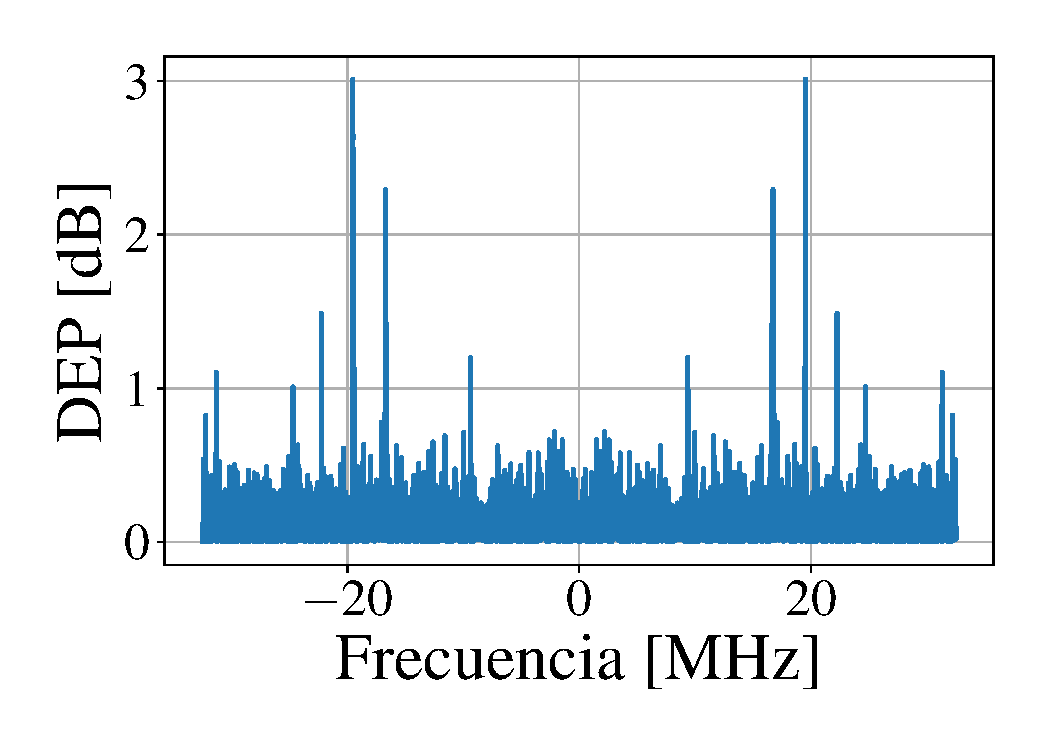
\includegraphics[width=0.49\linewidth]{tresTonosMuchoRuido-dataInFreq.pdf}}
    \hspace{\fill}%\\[1PC]
    \subcaptionbox{DEP de la salida del filtrado de banda.\label{fig::tresTonosMuchoRuido-bandFilterFreq}}
    {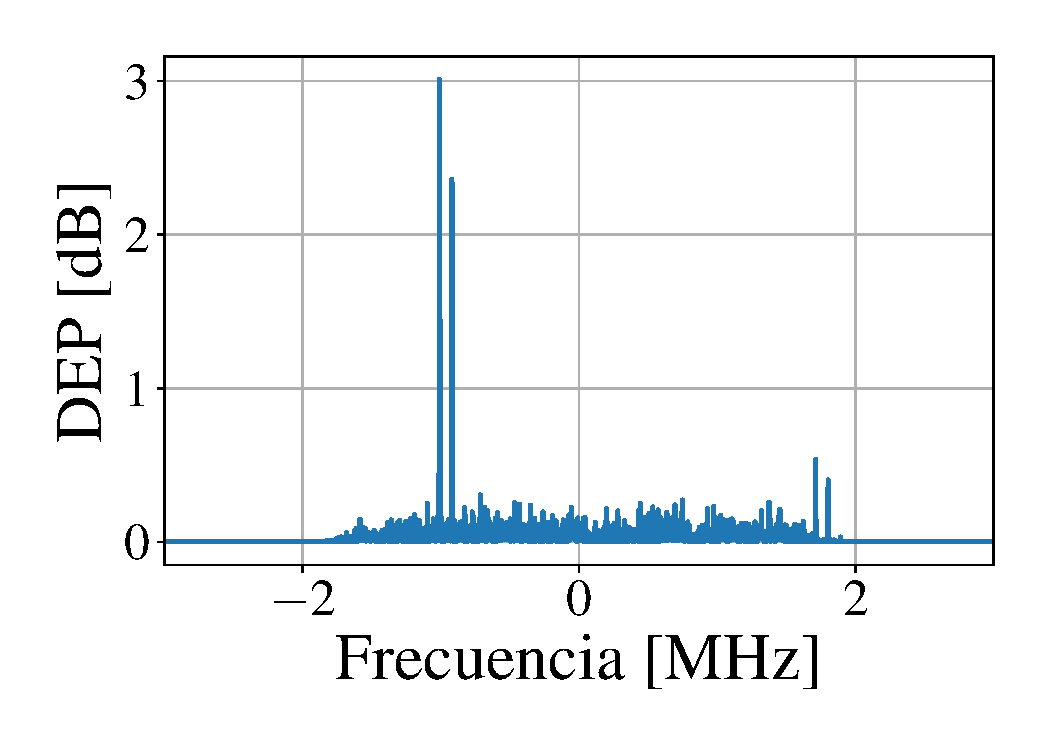
\includegraphics[width=0.49\linewidth]{tresTonosMuchoRuido-bandFilterFreq.pdf}}
    \\[1PC]
    \subcaptionbox{DEP de la salida del filtrado de haz.\label{fig::tresTonosMuchoRuido-channelFreq}}
    {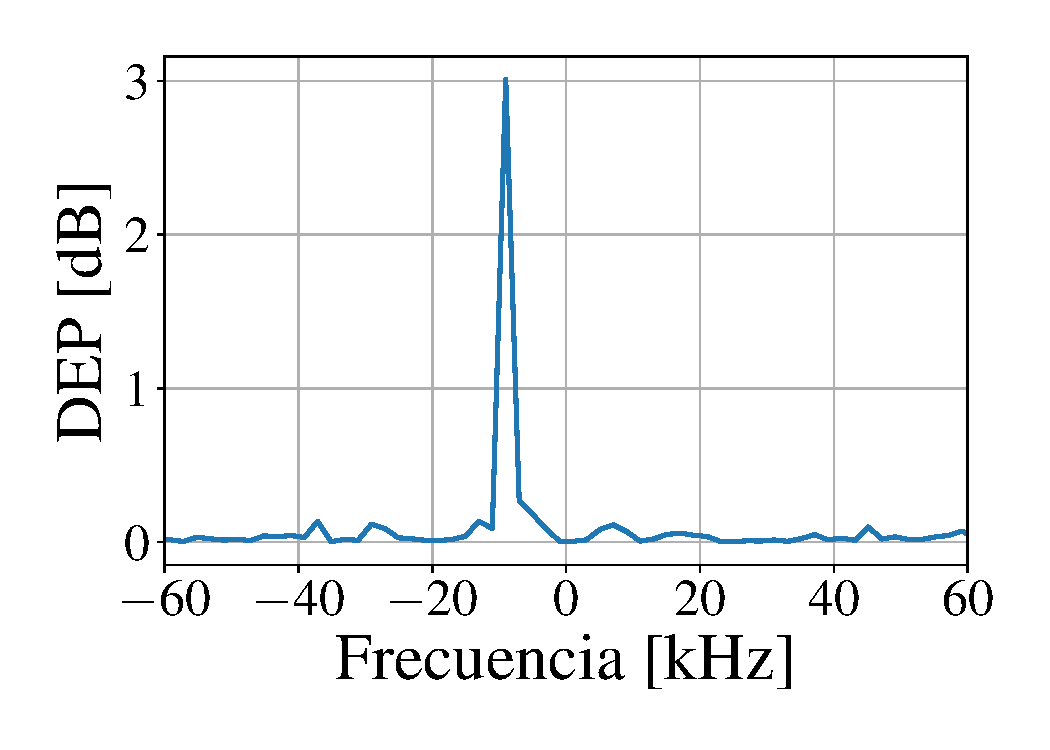
\includegraphics[width=0.49\linewidth]{tresTonosMuchoRuido-channelFreq.pdf}}
    \caption{Resultados de la simualación enviando tres tonos con ruido por el agente ADC.}
    \label{fig::tresTonosMuchoRuido}
\end{figure}

\section{Integración con el sistema de adquisición}
Habiendo desarrollado y validado la etapa de preprocesamiento de manera aislada (\textit{standalone}), se procede a realizar la integración con el \textit{core} de adquisición desarrollado en~\cite{proyecto-jose}.

Todo el código relacionado con la integración de los proyectos se encuentra en el submódulo \texttt{PIQuinteros/} del respositorio, en las ramas \texttt{dev-fran} y \texttt{dev-fran-opt} ya que se extendió directamente el proyecto existente, que se ubica dentro de ese repositorio. Más especificamente, se encuentra en el directorio \texttt{PIQuinteros/Fpga/}

\subsection{Recreación del proyecto preexistente}
Para lograr la integración de la etapa de preprocesamiento con el proyecto llevado a cabo en~\cite{proyecto-jose}, resulta necesario entender los aspectos más importantes del mismo. Para esto se recreó el proyecto original con los archivos ubicados en la rama \texttt{main} del submódulo.

Se empleó \textit{Vivado} para generar el \textit{bitstream}, esto es, el archivo de configuración de la FPGA correspondiente al proyecto y \textit{Vitis Unified Software Platform} para generar los archivos binarios a correr en el PS y en una computadora externa.

Un diagrama de lo implementado dentro de la CIAA-ACC en~\cite{proyecto-jose} se muestra en la figura \ref{fig::pipeline-ciaa}, a excepción de la etapa de preprocesamiento, la cual no se implementó en dicho proyecto.

Se logró exitósamente replicar los resultados mostrados en~\cite{proyecto-jose}, transmitiendo y recibiendo capturas utilizando el software allí desarrollado.

\subsection{Módulos y IPs empleados en la integración}
En las tablas \ref{tab::ip-vivado-integracion} y \ref{tab::ip-fran-integracion} se mencionan los \textit{IP cores} empleados durante la integración, además de los ya mencionados en las tablas \ref{tab::ip-vivado-preproc} y \ref{tab::ip-fran}, los cuales fueron reutilizados en este proyecto.

El objetivo de las tablas recién mencionadas es agrupar todos los IPs desarrollados, sin embargo, su funcionamiento se explicará en mayor detalle a medida que los mismos surjan en la explicación del sistema que se dará en las secciones subsiguientes.
%FIFO Generator
%Clocking Wizard

%pulse_sync
%sampler_with_ce

\begin{table}[H]
    \centering
    \resizebox{0.9\textwidth}{!}{%
    \begin{tabular}{|llc|}
    \hline
    \multicolumn{3}{|c|}{\textbf{IPs nativas utilizadas en la integración del preprocesamiento}}                                                                                                                                                                                                                                                        \\ \hline
    \multicolumn{1}{|l|}{\textbf{Nombre}}    & \multicolumn{1}{l|}{\textbf{Función}}                                                                                                                                                                                  & \textbf{Documentación}                   \\ \hline
    \multicolumn{1}{|l|}{\texttt{Clocking Wizard}}   & \multicolumn{1}{l|}{\begin{tabular}[c]{@{}l@{}}Simplifica la generación de código\\para la especificación de circuitos de reloj personalizados.\end{tabular}}                                &~\cite{clk-wizard} \\ \hline
    \multicolumn{1}{|l|}{\texttt{Binary Counter}} & 
    \multicolumn{1}{l|}{Contador binario.}
    &~\cite{binary-counter}     \\ \hline
    \multicolumn{1}{|l|}{\texttt{FIFO Generator}}       & \multicolumn{1}{l|}{Implementa una cola FIFO.}                                                                                                                                                                      &~\cite{fifo-generator}     \\ \hline

    \end{tabular}%
    }
    \caption{IPs nativas utilizadas en la integración con el proyecto preexistente.}
    \label{tab::ip-vivado-integracion}
    \end{table}

\begin{table}[H]
\centering
    \resizebox{0.95\textwidth}{!}{%
    \begin{tabular}{|ll|}
    \hline
    \multicolumn{2}{|c|}{\textbf{Módulos desarrollados para la integración}}       \\ \hline
    \multicolumn{1}{|l|}{\textbf{Nombre}}                                                   & \textbf{Función}                                                                                                                                                        \\ \hline
    \multicolumn{1}{|l|}{\texttt{AXI 16 Reg Block}}                                                      & Bloque de 16 registros de tipo AXI4-Lite.                                                                                                                                                                \\ \hline
    \multicolumn{1}{|l|}{\texttt{AXI Joiner}}                                                    & Concatena y actualiza las salidas filtradas de los múltiples \textit{beams}.                                                                                                                                                                                                                                                                                                                                                                                                                      \\ \hline
    \multicolumn{1}{|l|}{\texttt{Beam Handler}}                                                   & \begin{tabular}[c]{@{}l@{}}Se encarga del manejo de los haces, incorporando\\ numerosas optimizaciones.\end{tabular}                                                                                                                                                                                    \\ \hline
    \multicolumn{1}{|l|}{\texttt{Beam Mux FSM}}                                                     & \begin{tabular}[c]{@{}l@{}}Máquina de estados finita para la multiplexación \\ temporal de los distintos \textit{beams} manteniendo el dato de entrada válido.\end{tabular}                                                                                                                                                                                                                                                                                          \\ \hline
    \multicolumn{1}{|l|}{\texttt{Beam Sel Mux}}                                                   & Multiplexor para seleccionar el haz que quiere recibirse. 
                                \\ \hline
    
    \multicolumn{1}{|l|}{\texttt{Complex Conjugator}}       &
    Recibe una señal compleja y entrega la señal conjugada.
                     \\ \hline
    \multicolumn{1}{|l|}{\texttt{Copy Vec N Times}}                                                     & Replica N veces las señales de entrada tipo AXI4-Stream a la salida.  
    \\ \hline
    \multicolumn{1}{|l|}{\texttt{CRC 32}} & 
    Implementación del algoritmo de CRC-32.             
    \\ \hline
    
    \multicolumn{1}{|l|}{\texttt{Data Handler}}       &
    \begin{tabular}[c]{@{}l@{}}Bloque que sirve como abstracción para operar con las señales de\\ los 16 canales en el orden correcto y al mismo tiempo.\\ Toda la etapa de preprocesamiento y gran parte del sistema \\ preexistente se instanció sobre este bloque.\end{tabular}   
    \\ \hline
    
    \multicolumn{1}{|l|}{\texttt{FIFO Input Data Mux}}       &
    \begin{tabular}[c]{@{}l@{}}Multiplexor para seleccionar la entrada a las FIFOs\\ de datos, los cuales luego serán visualizables.\end{tabular}   
    
        \\ \hline
    
    \multicolumn{1}{|l|}{\texttt{Level Sync}}       &
    Sincronizador por nivel empleado en CDCs.
        \\ \hline
    
    \multicolumn{1}{|l|}{\texttt{Preprocessing}}                                                       & Módulo que instancia toda la lógica de preprocesamiento.  
   
       \\ \hline
           \multicolumn{1}{|l|}{\texttt{Pulse Sync}}       &
    Sincronizador de pulsos empleado en CDCs.
    
        \\ \hline
    
    
    \multicolumn{1}{|l|}{\texttt{Quasistatic Sync}}       &
    Sincronizador para señales lentas o cuasiestáticas empleado en CDCs.
    \\ \hline
    

    \multicolumn{1}{|l|}{\texttt{Sampler with CE}}       &
    Muestreador de una señal con una señal de \textit{clock enable}.


    \\ \hline
    
    \multicolumn{1}{|l|}{\texttt{Vector-valid Sync}}       &
    Sincronizador de interfaces de tipo AXI4-Stream con señal de datos y de \textit{valid}.


                                                                                         \\ \hline
    \end{tabular}%
    }
    \caption{Módulos desarrollados en VHDL para la integración de la etapa de preprocesamiento en el proyecto preexistente.}
    \label{tab::ip-fran-integracion}
    \end{table}

\subsection{Diferencias de interfaz}
La integración del presente proyecto con el \textit{core} de adquisición ya existente no resulta directa ya que existen diferencias que deben ser salvadas para poder lograr la incorporación de la etapa de preprocesamiento. Estas diferencias se mencionan en la tabla \ref{tab::diferencias-integracion}

%Clock a 260, CDCs
%División en varios bloques para minimizar replicas (16 canales)
%Aumento dato fifo (32 bits en lugar de 16)
%Uso de dos shorts como complex
%Uso de complemento a 2
%JQ: cambio a RTL top, corte de adc_receiver para poder usar única etapa de procesamiento, mejoras de timing...

\begin{table}[H]
    \centering
    \resizebox{0.8\textwidth}{!}{%
    \begin{tabular}{|l|c|c|}
    \hline
                                                                                   & \textbf{Proyecto preexistente} & \textbf{Etapa de preprocesamiento a integrar} \\ \hline
    \textbf{Frecuencia de reloj}                                                   & 65 MHz                         & 260 MHz                                       \\ \hline
    \textbf{Formato de datos}                                                      & Enteros de 16 bits             & Complejos de 32 bits en total                 \\ \hline
    \textbf{\begin{tabular}[c]{@{}l@{}}Ancho de datos\\ en las FIFOs\end{tabular}} & Dos datos de 16 bits           & Un dato de 32 bits                            \\ \hline
    \textbf{Cantidad de canales}                                                   & 16                             & 1                                             \\ \hline
    \end{tabular}%
    }
    \caption{Diferencias a salvar para lograr la integración de la etapa de preprocesamiento.}\label{tab::diferencias-integracion}
    \end{table}

La adaptación del formato de datos y el ancho de las FIFOs resulta directa ya que el \textit{core} de adquisición fue diseñado de manera de trabajar con dos datos de 16 bits ya que el ancho de los registros del bus AXI fue fijado a 32 bits. La transición de 16 a 32 bits se lleva a cabo en las colas FIFO, las almacenan los datos capturados para luego ser leídos por el PS mediante el bus AXI.

La instanciación de las colas FIFO se hace a través del IP \texttt{FIFO Generator} de Xilinx~\cite{fifo-generator}. Este IP provee la configuración de los parámetros \textit{Input Data Width} y \textit{Output Data Width}, los cuales en el \textit{core} de adquisición fueron configurados como 16 y 32 bits respectivamente.

De esta manera, la única adaptación necesaria consiste es aumentar el parámetro \textit{Input Data Width} del IP \texttt{FIFO Generator} a 32 bits para poder escribir a las FIFOs datos complejos.

La diferencia mostrada en la tabla \ref{tab::diferencias-integracion} que queda por resolver es la de la frecuencia de reloj para el preprocesamiento de los datos. Dado que toda la etapa de preprocesamiento \textit{standalone} se desarrolló con el reloj de 260~MHz, lo más conveniente es adaptar el \textit{core} de adquisición para poder operar a esta frecuencia.

Como se mencionó en la ecuación \ref{eq::DCO}, el ADC opera con una frecuencia de reloj de datos de 455~MHz. Esta es la frecuencia a partir de la cual se genera la nueva señal de reloj a 65~MHz en el proyecto preexistente mediante la instanciación del IP \texttt{Clocking Wizard}. Para cambiar la frecuencia de trabajo entonces se removió dicha instancia y se generó una nueva, la cual, a partir del reloj de 455~MHz genera una nueva señal de \textit{clock} de 260~MHz.

Finalmente, en cuanto a la discrepancia en número de canales, se optó en primera instancia por replicar la lógica de la etapa de preprocesamiento 16 veces. Esto se optimizará más adelante tras avanzar en la integración de los proyectos.

\subsection{Cruces de dominio de reloj (CDCs)}\label{subsec::cdcs-integracion}
Existen en el diseño tres dominios de reloj distintos:
\begin{itemize}
    \item El del ADC, el cual tiene una frecuencia de 455~MHz.
    \item El del preprocesamiento a 260~MHz.
    \item El de las interfaces AXI, a 100~MHz.
\end{itemize}
Como consecuencia de esto, se vuelve necesario determinar mecanismos para la sincronización de señales que atraviesen de un dominio a otro. Se evalúan a continuación todos estos casos y se desarrolla el método de CDC adecuado.
%constraints - false paths
%Raw data path para calibracion
%Cambio de índices
%Fifo input mux
\subsubsection{Sincronización de datos del deserializador}
Ya con el nuevo reloj de 260~MHz generado, se vuelve necesario sincronizar los datos de salida del deserializador, el cual entrega datos de 14~bits a 65~MSps como, esto es, a la máxima frecuencia de muestreo del ADC (ver tabla~\ref{tab::ADC}) y opera en el dominio de reloj del ADC (455~MHz). Esto se realizó en dos partes de la siguiente manera:
\begin{enumerate}
    \item Se sincronizó el pulso de \textit{valid} proveniente del deserializador, el cual se encuentra en el dominio de reloj de 455~MHz. 
    \item Se muestreó la salida del deserializador con el pulso de \textit{valid} ya sincronizado al dominio de reloj de 260~MHz.
\end{enumerate}

Para el primer punto se instanció el módulo \texttt{Pulse Sync}, mencionado en la tabla \ref{tab::ip-fran-integracion}, el cual sincroniza un pulso de un dominio de reloj a otro. Su funcionamiento se ilustra en la figura~\ref{fig::pulse-sync}.

Con el pulso de \textit{valid} ya sincronizado, se procedió a muestrear la señal de datos proveniente del deserializador mediante la instanciación del módulo \texttt{Sampler with CE}, el cual muestrea una señal al recibir un pulso de \textit{clock enable}, el cual en este caso corresponde al pulso de \textit{valid} recién sincronizado.

\figura[0.8]{pulse-sync}{Estructura del sincronizador de pulsos entre dos dominios de reloj.}

\subsubsection{Sincronización de señales de control}
%Sync de vector quariestático para señales de control
Para lograr el CDC en las señales de control como por ejemplo la que selecciona la salida del \texttt{Data Source Mux}, cuyo dominio de reloj es el del \texttt{AXI Interconnect} se instanció el módulo \texttt{Quasistatic Sync}, el cual implementa un sincronizador para señales cuasiestáticas como el mostrado en la figura \ref{fig::CDC-preproc}. La explicación para la sincronización de este tipo de señales es la ya dada en la subsección \ref{subsec::cdcs-standalone}.

\subsubsection{Sincronización de señales por nivel}
%Sync de nivel para la señal de debug y de la fifo
Señales por nivel, como la señal de \textit{full} de las colas FIFO, se sincronizaron con el módulo \texttt{Level Sync}, el cual consiste en un registro de desplazamiento con $N$ \textit{flip flops} de profundidad, siendo $N$ un parámetro configurable.

\subsubsection{Sincronización para interfaces AXI4-Stream cuasiestáticas}
%Sync de AXI (data vector + valid) para el local osc freq y las señales de frec en gral
En el caso de la sincronización de interfaces AXI4-Stream compuestas por una señal de datos y una de \textit{valid} puede aplicarse la misma técnica de sincronización del pulso de \textit{valid} y muestreo con \textit{clock enable} que se desarrolló en anteriormente para el caso de la salida del deserializador. Un mecanismo similar a este que utiliza 3 \textit{flip flops} para estabilizar la señal de \textit{valid} se implementó en el módulo \texttt{Vector-valid Sync}.


Todas estas técnicas de CDC fueron aplicadas en el proceso de integración de la etapa de preprocesamiento. Se hará referencia a ellas a medida que surjan en el desarollo.



\subsection{Adaptación de los \textit{constraints} del proyecto}
Las \textit{constraints} o restricciones de diseño definen los requisitos que debe cumplir el flujo de compilación en \textit{Vivado} para que el diseño sea funcional en la placa~\cite{xdc-constraints}. En \textit{Vivado}, estos se especifican mediante un archivo de texto con extensión \texttt{.xdc} (\textit{Xilinx Design Constraints}), en el cual todos los \textit{constraints} se especifican mediante comandos de TCL (lenguaje de \textit{scripting}).

El proyecto preexistente ya implementa un archivo XDC en el cual se especifican las asociaciones de puertos con pines de la FPGA (llamado \textit{pinout}) y se fijan estándares eléctricos entre otras cosas. Estos archivos se encuentan en \texttt{PIQuinteros/Fpga/src/constraints/}.

En dicho directorio se incorporó un nuevo archivo llamado \texttt{ciaa\_acc\_SistAdq\_timing.xdc}. En este archivo se especificaron \textit{constraints} relacionados al \textit{timing} del sistema. En particular, se empleó el comando \texttt{set\_false\_path} para que \textit{Vivado} ignore ciertos \textit{caminos} a la hora de realizar el análisis de \textit{timing}~\cite{false-paths}.

Los caminos a ser ignorados por la herramienta están son aquellos que incurren en un CDC, ya que estos casos fueron debidamente abordados empleando lógica adicional de sincronización para evitar problemas de metaestabilidad. 

En general, las señales involucradas en los CDCs son lentas o cuasiestáticas como se desarrolló en la subsección \ref{subsec::cdcs-integracion}, a excepción de la señal de datos que sale del deserializador. 

En este caso particular se tienen datos generados a 65~MSps empleando un reloj de 455~MHz, los cuales deben muestrearse a medida que salen con el reloj de 260~MHz. De manera,que se dispone de 4 ciclos del reloj de 260~MHz para muestrear la señal que sale del deserializador. Sin embargo, también debe considerarse que el módulo \texttt{Pulse Sync} hace uso de 2 ciclos de reloj para sincronizar la señal de \textit{valid}, la cual luego se utilizará como \textit{clock enable} para el módulo \texttt{Sampler with CE} (ver subsección \ref{subsec::cdcs-integracion}). Como consecuencia, la señal de datos proveniente del deserializador debe estar estable para ser muestreada luego de 2 ciclos de reloj de 260~MHz.

Este requerimiento puede expresarse en el archivo XDC a través de la función \texttt{set\_max\_delay}, la cual permite fijar un retraso máximo para un dado \textit{datapath}~\cite{set-max-delay}. En este caso, dicho retraso máximo es de $1000 \cdot 2/260\un{ns}$.

\section{Refactorización del código preexistente}
%Simplificación del adc_receiver
%Eliminación del bd_top para poder instanciar bds
%Incorporación del data_handler
%Ordenamiento natural de los canales
Durante la integración de la etapa de preprocesamiento con el \textit{core} de adquisición se realizó una refactorización del código desarrollado en el sistema de adquisición original con el objetivo de simplificar la estructura del mismo y optimizar el uso de recursos dentro de la FPGA.

Para poder entender las modificaciones realizadas a la base de código y las subsecuentes optimizaciones resultantes, es necesario primero familiarizarse con algunos aspectos relevantes de la implementación original del \textit{core} llevada a cabo en~\cite{proyecto-jose}, los cuales se mencionan a continuación:
\begin{enumerate}
    \item El módulo principal del sistema (\textit{top module}) se instancia dentro de un diagrama de bloques o \textit{block design} generado mediante el \textit{Vivado IP Integrator}~\cite{vivado-ip-integrator}.
    \item Parte de la lógica se repite en dos instancias del módulo \texttt{ADC Receiver}.
\end{enumerate}

La relevancia del primer punto mencionado radica en que la versión 2020.2 de \textit{Vivado} utilizada en este proyecto no permite anidar diagramas de bloques. Es decir, no es posible instanciar un diagrama de bloques dentro de otro. En consecuencia, dado que la etapa de preprocesamiento diseñada en \ref{subsec::implementacion-vivado} fue implementada en un \textit{block design}, fue necesario transcribir el módulo \textit{top} a un módulo de VHDL. El mismo se encuentra en \texttt{PIQuinteros/Fpga/src/hdl/SistAdq\_top.vhd}.

El módulo \texttt{ADC Receiver}, ubicado en \texttt{PIQuinteros/Fpga/src/hdl/adc\_receiver.vhd}, contiene la lógica de los retardos de entrada y el deserializador, entre otras cosas. Este módulo se instancia dos veces debido a que, en el \textit{mapeo} de pines del conector FMC, de los 16 canales de datos del ADC, 14 se encuentran en el banco 12 de la FPGA y 2 en el banco 13 de esta (para mayor detalle ver \cite{proyecto-jose}).

Originalmente, en el módulo \texttt{ADC Receiver} se instanciaba no solo a los retardos de entrada y el deserializador, sino también las herramientas de \textit{debug} desarrolladas en el proyecto del \textit{core} de adquisición junto con las colas FIFO. Más aún, en una primera incorporación de la etapa de preprocesamiento, la misma se instanció también dentro del módulo \texttt{ADC Receiver}, lo cual implicaba la replicación de aún más lógica. Viendo la figura \ref{fig::pipeline-ciaa}, en líneas generales, toda la lógica desde los retardos de entrada hasta las FIFO estaba instanciada en este módulo.

Se propuso entonces mantener las dos instancias del \texttt{ADC Receiver} pero minimizando el contenido de las mismas. De esta manera, solo se conservó en este módulo la lógica relacionada a los retardos de entrada y el deserializador.

Se creó un nuevo módulo en VHDL llamado \texttt{Data Handler}, el cual sirvió como unificador de las 16 señales de datos ya que procesaba en conjunto y de forma ordenada todos los canales del ADC. Resulta relevante destacar el ordenamiento de los canales ya que los dos canales que se encuentran en el banco 13 de la FPGA son los canales 11 y 16, de manera que las señales de salida los dos \texttt{ADC Receiver} deben ser reordenadas. Este reordenamiento se explicita en la tabla \ref{tab::reordenamiento-adc-receivers}.

\begin{table}[H]
    \centering
    \resizebox{0.8\textwidth}{!}{%
    \begin{tabular}{|c|c|c|c|}
    \hline
     & \textbf{Entrada al} \texttt{Data Handler} & \textbf{Salida del} \texttt{ADC Receiver 1} & \textbf{Salida del} \texttt{ADC Receiver 2} \\ \hline
    \multirow{16}{*}{\textbf{\begin{tabular}[c]{@{}c@{}}Número de\\ canal\end{tabular}}} & 1 & 1 & - \\ \cline{2-4} 
     & 2 & 2 & - \\ \cline{2-4} 
     & 3 & 3 & - \\ \cline{2-4} 
     & 4 & 4 & - \\ \cline{2-4} 
     & 5 & 5 & - \\ \cline{2-4} 
     & 6 & 6 & - \\ \cline{2-4} 
     & 7 & 7 & - \\ \cline{2-4} 
     & 8 & 8 & - \\ \cline{2-4} 
     & 9 & 9 & - \\ \cline{2-4} 
     & 10 & 10 & - \\ \cline{2-4} 
     & 11 & - & 1 \\ \cline{2-4} 
     & 12 & 11 & - \\ \cline{2-4} 
     & 13 & 12 & - \\ \cline{2-4} 
     & 14 & 13 & - \\ \cline{2-4} 
     & 15 & 14 & - \\ \cline{2-4} 
     & 16 & - & 2 \\ \hline
    \end{tabular}%
    }
    \caption{Asignación de canales de datos del \texttt{Data Handler} a partir de la salida de ambas instancias del \texttt{ADC Receiver}.}\label{tab::reordenamiento-adc-receivers}
    \end{table}

Dentro del \texttt{Data Handler} se instanció la etapa de \textit{debug} desarrollada en \cite{proyecto-jose} junto con toda la lógica relacionada con el preprocesamiento, abstraída en un archivo aparte, el cual puede encontrarse en \texttt{PIQuinteros/Fpga/src/hdl/preprocessing.vhd}. Finalmente, las colas FIFO también fueron trasladadas a este módulo.

\section{Modificaciones y ampliaciones}
Durante la integración de los proyectos se realizaron ampliaciones al funcionamiento del sistema en general como por ejemplo la extensión de las herramientas de \textit{debug} o la incorporación de múltiples \textit{beams} como se describirá a continuación.

\subsection{Ajuste de la precisión en el incremento de fase}
En el diseño \textit{standalone} de la etapa de preprocesmiento se empleó $N = 16\un{bits}$ en el cálculo del incremento de fase detallado en la ecuación \ref{eq::calculo-incremento-fase-v2}. Con esa cantidad de bits, la resolución de frecuencia reportada por el \texttt{DDS Compiler} con el reloj de 260~MHz es de $3.9\un{kHz}$. Este valor resulta demasiado alto considerando que el ancho de banda de los haces a ser seleccionados es de 25~kHz.

Luego, se incrementó la cantidad de bits empleados en la definición del incremento de fase a 32. Con el \textit{clock} de 260~MHz, la resolución reportada por el \texttt{DDS Compiler} es $2^{16}$ veces mejor, esto equivale a una resolución de $0.06\un{Hz}$.

\subsection{Ampliación de las herramientas de \textit{debug}}
En la subsección \ref{subsec::debug-preproc-inicial} se mencionó la inclusión del módulo \texttt{Data Source Mux} como herramienta de \textit{debug} para seleccionar la entrada de datos ya sea desde el ADC, desde un oscilador de frecuencia conocida o un contador.

Durante la integración del \textit{core} de adquisición con la etapa de preprocesamiento no solo se mantuvo este módulo, sino que se incluyó además un nuevo módulo, llamado \texttt{FIFO Input Mux} para facilitar el acceso al usuario a distintos puntos del sistema.

El \texttt{FIFO Input Mux} es, como su nombre lo indica, un multiplexor que permite seleccionar la señal de entrada a las colas FIFO, y así otorga al usuario la posibilidad de observar las señales en diversos puntos del sistema. Las configuraciones posibles se muestran en la tabla \ref{tab::fifo-input-mux}.

El multiplexor se controla mediante una señal asociada al registro~43C30004, con lo cual debe ser sincronizada de manera acorde como una señal de control según se explicó en \ref{subsec::cdcs-integracion}.

\begin{table}[H]
\centering
\resizebox{\textwidth}{!}{%
\begin{tabular}{|lll|}
\hline
\multicolumn{3}{|l|}{\texttt{FIFO Input Mux} \textbf{-- Dirección de registro: 43C30004}}        \\ \hline                                                                                     
\multicolumn{1}{|l|}{\textbf{Valor}} & \multicolumn{1}{l|}{\textbf{Selección}} & \textbf{Descripción}                                                                                                                                      \\ \hline
\multicolumn{1}{|l|}{0}              & \multicolumn{1}{l|}{Desactivado}        & No se envía nada a las FIFOs.                                                                                                                             \\ \hline
\multicolumn{1}{|l|}{1}              & \multicolumn{1}{l|}{Preprocesamiento}   & \begin{tabular}[c]{@{}l@{}}Se asigna la salida de la etapa de preprocesamiento \\ a la entrada de las FIFOs.\end{tabular}                                 \\ \hline
\multicolumn{1}{|l|}{2}              & \multicolumn{1}{l|}{Datos crudos}       & \begin{tabular}[c]{@{}l@{}}Selecciona datos crudos del ADC, estos son los datos \\ que salen directamente del deserializador.\end{tabular}                \\ \hline
\multicolumn{1}{|l|}{3}              & \multicolumn{1}{l|}{Contador}           & Se asigna la salida de un contador.                                                                                                                       \\ \hline
\multicolumn{1}{|l|}{4}              & \multicolumn{1}{l|}{Mezclador de banda} & \begin{tabular}[c]{@{}l@{}}La salida del módulo bajo esta configuración son los \\ datos de salida de la primera mezcla de preprocesamiento.\end{tabular} \\ \hline
\multicolumn{1}{|l|}{5}              & \multicolumn{1}{l|}{Filtrado de banda}  & Los datos de salida se corresponden con la salida del filtro de banda.                                                                                    \\ \hline
\multicolumn{1}{|l|}{6}              & \multicolumn{1}{l|}{Mezclador de haz}   & La entrada a las FIFOs es la salida del mezclador de haz.                                                                                                 \\ \hline
\end{tabular}%
}
\caption{Valores de configuración y salidas del \texttt{FIFO Input Mux}}\label{tab::fifo-input-mux}
\end{table}

\subsubsection{Incorporación de CRC-32}
Se incorporó dentro de la FPGA el módulo \texttt{CRC 32} el cual calcula el CRC-32 de acuerdo al estándar IEEE~802.3\todo{ref}. La implementación del mismo en VHDL se extrajo de \cite{crc-impl}.

La instancia del módulo \texttt{CRC 32} se ubica en la cercanía de la interfaz entre PS y PL ya que cada dato leído en una FIFO se envía al módulo como entrada al CRC junto con una señal de \textit{enable}. Esto es, al recibirse la señal de \textit{read enable} en un registro de datos de la FPGA, esta sirve como señal de \textit{enable} para el módulo del CRC, al cual también se le entrega el dato que está siendo leído.

De esta manera, todos los datos de las colas FIFO forman parte del CRC calculado, el cual finalmente se almacena en otro registro para ser leído por el software. Una vez realizada la lectura del mismo, se \textit{resetea} su valor antes de comenzar la adquisición de un nuevo paquete.

Se modificó el código base para incluir dos señales de \textit{reset}. La primera corresponde a la señal de \textit{reset} inicial al encender el sistema, mientras que la segunda señal se utiliza para \textit{resetear} el cálculo del CRC para cada nuevo paquete. 

\subsection{Configuración de frecuencia y sentido de rotación del espectro}\label{subsec::config-frec}
El oscilador de haz implementado en la subsección \ref{subsec::implementacion-vivado} se configuró a una frecuencia fija de operación $f_\textrm{out}$ de 1~MHz como se mencionó en la tabla \ref{tab::osciladores-conf-preproc} para realizar la prueba de concepto y las simulaciones con UVM en la sección \ref{sec::simu-uvm}. Este parámetro, sin embargo, al ser el que selecciona el haz de interés, debe ser configurable por el usuario.

La configuración del oscilador puede hacerse configurando el parámetro \textit{Phase Increment Programmability} al valor \textit{Programmable} en el IP \textit{DDS Compiler} (ver tabla \ref{tab::ip-vivado-preproc}). Esto habilita una nueva interfaz de entrada de tipo AXI4-Stream al IP, como se muestra en la figura \ref{dds-programmable}. A través de esta interfaz puede configurarse un nuevo valor de incremento de fase según la ecuación \ref{eq::calculo-incremento-fase-v2}.

Luego, mediante la asignación de un registro del \texttt{AXI 16-Register Block} puede controlarse la frecuencia de oscilación del \texttt{DDS Compiler}. Por otro lado, también debe proveerse un pulso de \textit{valid}. Este puede tomarse directamente del pulso de \textit{write enable} que recibe el bloque de registros, parte del protocolo AXI4-Stream, el cual permite la escritura del registro. En otras palabras, cuando el registro de frecuencia se escribe, se habilita el pulso de \textit{valid}, el cual dura un solo ciclo de reloj.

La capacidad de configurar la frecuencia durante la operación se agregó también al oscilador local de \textit{debug}, el cual originalmente operaba a una frecuencia fija de $19.51\un{MHz}$, como se aclaró en la tabla\ref{tab::osciladores-conf-preproc}.

Por último, al tratarse de señales provenientes de distintos dominios de reloj, debe manejarse el CDC, en este caso al tratarse de una interfaz AXI4-Stream cuasiestática, se empleó el módulo \texttt{Vector-Valid Sync} como se explicó en la subsección \ref{subsec::cdcs-integracion}.

\figura[0.5]{dds-programmable}{\texttt{DDS Compiler} con interfaz AXI4-Stream para la programación del incremento de fase.}

\subsubsection{Sentido de rotación del espectro}
Una consideración que no se tuvo en cuenta en el diseño \textit{standalone} de la etapa de preprocesamiento es el sentido de rotación del espectro, es decir, el signo del exponente de la exponencial compleja utilizada para la mezcla.

Esto no es de relevancia en la primera mezcla, ya que el módulo del espectro es simétrico respecto a $f=0$ ya que las señales de entrada al ADC son reales. No obstante, tras la primer mezcla se tiene una copia de la banda de 3~MHz de UHF en banda base, la cual puede no ser simétrica respecto a $f= 0$.\footnote{Y seguramente no lo sea.}

Una consecuencia directa de este hecho es que a la hora de realizar la segunda mezcla se vuelve necesario poder seleccionar el sentido de la rotación del espectro. Esto se puede ver claramente en la figura \ref{fig::espectro-canal}, donde se observa que, al no se simétrico el módulo del espectro, realizar una traslación de 1~MHz no resulta equivalente a realizar una de -1~MHz.

El sentido de rotación del espectro está determinado por el signo del exponente de la exponencial compleja generada por el \texttt{DDS Compiler} del oscilador de canal. Esto se puede cambiar mediante la configuración del parámetro \textit{Polarity}, sin embargo, este parámetro no es reconfigurable durante operación. 

Como solución a esto se creó un nuevo IP en VHDL llamado \texttt{Complex Conjugator}, el cual recibe la exponencial compleja de salida del \texttt{DDS Compiler Controller} (el cual está en una jerarquía junto con un \texttt{DDS Compiler}, como la mostrada en la figura \ref{fig::local-osc}) y, mediante una señal de control, se encarga controlar el sentido de la rotación. 

La operación del \texttt{Complex Conjugator} se basa en el hecho de que
\[e^{j\theta} = \cos(\theta) + j \ \sin(\theta),\] y \[e^{-j\theta} = \cos(\theta) - j \ \sin(\theta).\] Luego, todo lo que se necesita para controlar el sentido de la rotación es controlar el signo de la parte imaginaria de la señal generada por el \texttt{DDS Compiler}.

De igual manera que se hizo con la señal de configuración de frecuencia, se asocio un registro a la señal de control de sentido de rotación y se manejo su señal de \textit{valid} de la misma manera, esto es, utilizando el pulso de \textit{write enable} como señal de \textit{valid}. Por último, nuevamente se manejó el CDC con un módulo \texttt{Vector-Valid Sync}.

Tras esta incorporación, el sistema ya es capaz de sintonizar un haz centrado a cualquier frecuencia dentro de la banda amateur para satélites en UHF.

\figura[0.7]{bd-beam-osc}{Diagrama de bloques del oscilador de canal incoporando el \texttt{Complex Conjugator}.}

\subsection{Modificaciones a los filtros}
Se modificaron las configuraciones de los filtros mostradas en la tabla \ref{tab::filtros-preproc}. Los cambios realizados fueron los siguientes:
\begin{itemize}
    \item Se aumentó la tasa de decimación de los filtros de banda de un factor 8 a un factor 10.
    \item Se aumentó la tasa de decimación de los filtros de haz de un factor 50 a un factor 100.
    \item Se redujeron la frecuencia de paso y de rechazo de los filtros de canal a 25~kHz y 32~kHz respectivamente. Provocando un aumento en el orden del filtro a 615\change{Este no es el orden final}.
\end{itemize}

En la tabla \ref{tab::filtro-beam-nuevo} se muestran las especificaciones relevantes de los filtros, mientras que en la figura \ref{fig::filtro-beam-nuevo} se muestra la respuesta en frecuencia y las especificaciones del filtro de haz, el cual se diseño con la herramienta \texttt{Filter Designer}\cite{filter-designer}.

El aumento en la tasa de decimación de los filtros se realizó por dos motivos:
\begin{enumerate}
    \item Mientras se siga cumpliendo con el teorema del muestreo, disminuir la tasa de muestras representa una disminución en el procesamiento sin pérdida de información.
    \item Disponer de más ciclos de reloj entre datos válidos da lugar a reutilización de recursos mediante multiplexación temporal como se discutirá oportunamente en la sección \ref{sec::optimizaciones}.
\end{enumerate}

Por otro lado, las nuevas frecuencias de paso y rechazo para los filtros de haz se eligió de manera tal de permitir el paso de una señal de 25~kHz de ancho de banda corrida hasta aproximadamente 10~kHz por efecto Doppler, como se describió en la sección \ref{sec::doppler}. Además, dado que la tasa de datos a la salida del filtro de haz es de 65~kHz, debe asegurarse que la frecuencia de rechazo sea menor o igual a 32,5~kHz para evitar el aliasing.

\begin{table}[H]
    \centering
    \resizebox{0.7\textwidth}{!}{%
    \begin{tabular}{|l|c|c|}
    \hline
    \multicolumn{1}{|c|}{}                  & Filtro de banda & Filtro de haz \\ \hline
    Frecuencia de paso {[}kHz{]}            & 1500            & 25          \\ \hline
    Frecuencia de rechazo {[}kHz{]}         & 2000              & 32           \\ \hline
    Atenuación en banda de paso {[}dB{]}    & 0               & 0             \\ \hline
    Atenuación en banda de rechazo {[}dB{]} & 40              & 40            \\ \hline
    Tipo de filtro                          & Equirriple      & Equirriple    \\ \hline
    Orden del filtro                        & 185             & 615           \\ \hline
    Frecuencia de muestreo {[}Msps{]}       & 65              & 6,5         \\ \hline
    Factor de decimación                    & 10               & 100            \\ \hline
    \end{tabular}%
    }
    \caption{Configuraciones principales de los nuevos filtros de banda y de haz.}
    \label{tab::filtro-beam-nuevo}
\end{table}
\change{Revisar Orden del filtro nuevo}


\figura[0.7]{filtro-beam-nuevo}{Diseño del nuevo filtro de haz considerando la nueva tasa de muestreo y la nueva definición de las frecuencias de paso y rechazo especificadas en la tabla \ref{tab::filtro-beam-nuevo}.}


\subsection{Incorporación de múltiples haces}\label{subsec::multiples-haces}
%Aces configurables, freq y signo
Una de las principales ventajas de la conformación de haz digital es, como se mencionó en el capítulo \ref{cap::intro}, la capacidad de realizar apuntamiento múltiple de manera simultánea. 

Para realizar el seguimiento de múltiples haces al mismo tiempo debe incorporarse un nuevo oscilador de \textit{beam} por cada nueva frecuencia que se desea seguir. Esto es así ya que el objetivo de oscilador de \textit{beam} es trasladar a banda base la señal de interés. En la figura \ref{fig::Multiples-beams} se muestra la arquitectura resultante para la etapa de preprocesamiento al incorporar múltiples \textit{beams}.

No obstante, si se quisieran adquirir todos los haces de manera simultánea debe incurrirse en cambios más fundamentales como la incorporación de más FIFOs y la modificación del software de adquisición desarrollado en \cite{proyecto-jose}. Dado que esta gran modificación no llegó a realizarse en este proyecto, se optó por incorporar 4 nuevos haces en la lógica para un total de 5 haces sintonizables y colocar un multiplexor a la salida de los filtros de haz (entrada del \texttt{FIFO Input Mux}) para seleccionar uno de los cinco \textit{beams} que se desea obtener a la salida.

Además, cada uno de estos osciladores de haz incorpora la capacidad de configurar su frecuencia y el sentido de rotación como se discutió en la subsección \ref{subsec::config-frec}.

\figura[0.8]{Multiples-beams}{Arquitectura del sistema para múltiples haces.}

\section{Optimizaciones}\label{sec::optimizaciones}
El diagrama para la incorporación de múltiples haces mostrado en la figura \ref{fig::Multiples-beams} es en realidad imposible de implementar de esa manera en la CIAA-ACC debido a la escasez de recursos. Esto hace necesaria la incorporación de técnicas de optimización de recursos. La realidad es que diversas optimizaciones se fueron implementando a lo largo del proceso, pero se decidió condensarlas todas juntas en esta sección para mayor claridad.

\subsection{Etapa de preprocesamiento}\label{subsec::preproc-opt}
El sistema de preprocesamiento admite grandes optimizaciones como reutilización de lógica o multiplexación temporal. Algunos IPs de Xilinx ya implementan esto como es el caso del \texttt{FIR Compiler}\cite{fir-compiler}.

Se refactorizó la etapa de preprocesamiento la cual, como se mencionó anteriormente se instanció dentro del módulo \texttt{Data Handler}. Esta refactorización tiene como objetivo también servir como una primera etapa de optimización de recursos dentro de la lógica programable. 

Para comenzar, el esquema implementado en el proyecto de preprocesamiento \textit{standalone}, mostrado en la figura \ref{fig::bd-preproc}, fue separado en cuatro partes con el objetivo de maximizar la reutilización de lógica. Estas partes son:
\begin{enumerate}
    \item \texttt{Preprocessing Setup BD}: Instancia el contador de \textit{debug}, el oscilador local a frecuencia conocida, el multiplexor de \textit{debug} y el oscilador de banda. Toda esta lógica solo debe instanciarse una vez. En la figura \ref{fig::bd-preprocessing-setup} se muestra este diagrama de bloques.
    \item \texttt{Band Processing BD}: Este BD debe instanciarse una vez por canal del ADC, es decir, debe replicarse 16 veces. El mismo instancia el \textit{zero padder} junto con el mezclador de banda y el filtro de banda. Este diagrama de bloques se muestra en la figura~\ref{fig::bd-band-processing}.
    \item \texttt{Beam Oscillator BD}: Debe instanciarse por cada frecuencia que desea sintonizarse, es decir, por cada \textit{beam} que quiera escucharse\footnote{Asumiendo que los \textit{beams} tienen todos frecuencias distintas.}. Este diagrama de bloques ya se mostró en la figura \ref{fig::bd-beam-osc}.
    \item \texttt{Beam Handler BD}: Se instancia una vez por canal del ADC, es decir, 16 veces. Este BD incluye grandes optimizaciones para el manejo de 5 haces simultáneos y su funcionamiento se explicará con más detalle a continuación.
\end{enumerate}

Es importante notar que el oscilador de banda instanciado en \texttt{Preprocessing Setup BD} será empleado como entrada a cada uno de los 16 mezcladores de banda, pero al tratarse siempre de una misma señal, no hay necesidad de instanciarlo 16 veces sino solo una.

Un cambio que puede observarse en la figura \ref{fig::bd-preprocessing-setup} es la incorporación del módulo \texttt{Copy Vec N Times}, que replica una entrada tipo interfaz AXI de \textit{data + valid} N veces a la salida, siendo N~=~16 en este caso. Esto resulta necesario ya que, debido a la integración de los 16 canales de datos del ADC con la incorporación del \texttt{Data Handler}, se eligió trabajar con una única gran señal de ancho $16\un{canales} \times 16\un{bits/canal} = 256\un{bits}$.

\figura[1]{bd-preprocessing-setup}{Diagrama de bloques \texttt{Preprocessing Setup BD}.}
\figura[1]{bd-band-processing}{Diagrama de bloques \texttt{Band Processing BD}.}

\subsection{Manejo de haces}\label{subsec::beam-handling}
Como se mencionó al principio de esta sección, es necesario optimizar el uso de recursos para lograr la incorporación de los cinco haces que se propuso implementar. Para esto se debe hacer un análisis de utilzación incial con el objetivo de identificar cómo se alocan los recursos en las diversas partes del preprocesamiento.

\subsubsection{Utilización con un único haz}
La primera implementación realizada, previa a la incorporación de los 5 haces, ya hacía uso de las optimizaciones listadas en \ref{subsec::preproc-opt} a excepción del \texttt{Beam Handler BD} dado que solo había un único haz. En este contexto, el resumen del reporte de utilización generado por \textit{Vivado} resultante es el mostrado en la figura \ref{fig::util-un-beam}. Allí se reporta la utilización de recursos como LUTs, FFs, BRAM y DSP \textit{blocks}, entre otros.

\figura[0.7]{util-un-beam}{Resumen del reporte de utilización para el sistema empleando un solo \textit{beam}.}

\subsubsection{Análisis de escalabilidad}
El objetivo que se propuso fue el de poder manejar 5 haces en simultáneo, con lo cual teniendo en cuenta la utilización de recursos para un único haz mostrada en la figura \ref{fig::util-un-beam}, debe analizarse el impacto en utilización que representa la incorporación de nuevos haces.

Para sintonizar una nueva frecuencia, según lo mostrado en la figura \ref{fig::Multiples-beams}, se requiere de un nuevo oscilador y un nuevo mezclador para trasladar a banda base, junto con un nuevo filtro a la salida de la mezcla. 

A continuación se analiza entonces el uso de recursos asociados a estos tres IPs.

\subsubsection{Oscilador de haz}
Cada oscilador de haz o \textit{beam}, al igual que el oscilador de banda instanciado del módulo \texttt{Preprocessing Setup BD}, solo debe instanciarse una única vez ya que su salida sirve de entrada a los mezcladores de los 16 canales. De esta manera, solo se necesita un oscilador por \textit{beam}, de manera que se requerirán 5 osciladores de haz, en lugar de $5\un{osciladores/canal} \times 16\un{canales} = 80\un{osciladores}$. Esto representa un factor 16 en la optimización de recursos.

El \textit{DDS Compiler} provee una estimación de recursos utilizados por el IP en la pestaña de información dentro de la ventana de configuración. En este caso, \textit{Vivado} reporta una utilización de 15 BRAM por parte de cada oscilador de \textit{beam}. Esto representa una utilización de \[15\un{BRAM/oscilador} \times 5\un{osciladores} = 75\un{BRAM},\] viendo el reporte de utilización previo a la incorporación de los 5 canales mostrado en la figura \ref{fig::util-un-beam}, este incremento en el uso de BRAMs no debería representar un inconveniente.

\subsubsection{Mezclador de haz}
Los mezcladores se implementaron empleando el IP \texttt{Complex Multiplier}, el mismo puede operar de con LUTs o DSPs. Al operar con DSPs, \textit{Vivado} da una estimación de 3 DSP \textit{blocks} utilizados por multiplicador. Por otro lado, al operar con LUTs no se provee una estimación de utilización. Sin embargo, para obtener un valor de referencia se reimplementó el proyecto con un solo haz empleando solo LUTs para los mezcladores. Al observar las diferencias en el reporte de utilización obtenido en la figura \ref{fig::util-un-beam} y dividiendo por la cantidad de multiplicadores se estimaron unas 844~LUTs por multiplicador.

Si se emplea un multiplicador por \textit{beam}, con 5 haces por canal y 16 canales, sumado al multiplicador de banda en cada uno de los 16 canales se requiere un total de \[5 \times 16 + 16 = 96\un{mezcladores}.\] Luego, empleando solo DSPs se necesitan \[3\un{DSP/mezclador} \times 96\un{mezcladores} = 288\un{DSPs}.\] Según el reporte de utilización de la figura \ref{fig::util-un-beam}, para un único haz ya se utilizan 196~DSPs, esto incluye a los mezcladores de canal y un único mezclador de haz, de manera al agregar los DSPs correspondientes a los 4 haces restantes se obtiene un total de \[196\un{DSPs} + 3\un{DSP/mezclador} \times 4\un{mezcladores/canal} \times 16\un{canales} = 388\un{DSPs}.\] Este valor es alcanzable por la placa, pero representa una utilización del 97\% de los DSP \textit{blocks}.

Por otro lado, si se decide usar LUTs, al tener 96~mezcladores donde cada uno ocupa 844~LUTs, se requerirían 81024~LUTs, valor que se encuentra por encima del máximo disponible según la figura \ref{fig::util-un-beam}.

Una solución más inteligente es, en lugar de instanciar los 96~\textit{mixers}, podría aprovecharse la baja tasa de datos en comparación a la frecuencia de reloj y realizar algún tipo de multiplexación temporal. De hecho, el reloj de preprocesamiento de 260~MHz ya de por sí es cuatro veces más rápido que el de datos, que es de 65~MHz. Pero además, tras la decimación en un factor 10 llevada a cabo en el filtrado de banda, la cantidad de ciclos de reloj incrementó de 4 a 40. Es decir, se tiene un total de 40 ciclos de reloj entre dos datos válidos, esto permite optimizar recursos mediante la reutilización de los recursos multiplexando en tiempo.

Con este objetivo, se creó el módulo \texttt{Beam Mux FSM}, el cual es una máquina de estados que se encarga del manejo de las señales a ser mezcladas en el \texttt{Complex Multiplier}. El objetivo es disponer de un único mezclador para cada canal, y así tener 32 mezcladores, 16 para la mezcla de banda y 16 para la de \textit{beam}, en lugar de los 96 que se calcularon inicialmente. Esto representa una mejora en un factor 3 en la utilización de recursos.

El módulo \texttt{Beam Mux FSM} es una máquina de estados que recibe la señal de salida del filtro de banda junto con todas las señales de los osciladores de haz. La salida de este módulo se compone de 4 señales:
\begin{itemize}
    \item \textit{Band filter data}: es la última señal de datos válida del filtro de banda. Se mantiene constante durante todos los estados, solo cambia con un nuevo \textit{valid} de entrada.
    \item \textit{Beam oscillator data}: es la señal del oscilador de \textit{beam} correspondiente. Este dato cambia en los distintos ciclos de reloj, multiplexando en tiempo los distintos osciladores de haz.
    \item \textit{Valid}: la señal de \textit{valid} es la proveniente del filtro de banda y se mantiene en alto una cantidad de ciclos igual a la cantidad de \textit{beams}, en este caso 5 ciclos. Luego se coloca en bajo.
    \item \textit{User}: se incorporó la señal de \textit{tuser} del estándar AXI4-Stream\cite{AXI-4-stream} para indicar el \textit{beam} al que corresponde cada salida de la FSM.
\end{itemize}

Al recibir un dato válido del filtro de banda, este módulo lo registra y lo mantiene como válido por 5 ciclos de reloj mientras multiplexa entre los distintas señales provenientes de los osciladores de \textit{beam}, indicando mediante el campo \textit{tuser} a que \textit{beam} corresponde cada señal.

Activando el uso del puerto campo \textit{tuser} en el IP \texttt{Complex Multiplier}, se puede conectar directamente las cuatro salidas del \texttt{Beam Mux FSM} a este sin mayores consideraciones. Es importante notar que usamos la misma señal de \textit{valid} para ambas entradas del mezclador, diferenciándolas mediante el uso del \textit{tuser}.

\subsubsection{\texttt{FIR Compiler}}
El IP tiene dos parámetros principales configurables para trabajar con múltiples haces, el número de canales y el número de caminos\cite{fir-compiler}. Este último ya se emplea a lo largo de toda la etapa de preprocesamiento para realizar el filtrado de una señal compleja.

Comprender la diferencia entre estos dos parámetros es fundamental. El número de caminos altera las interfaces de entrada y salida. Al tener dos caminos para una señal de entrada de 16~bits por ejemplo, el \texttt{FIR Compiler} espera a la entrada entonces una señal de $16 \times 2 = 32\un{bits}$. Por otro lado, el número de canales no altera las interfaces de entrada y salida, sino que realiza multiplexación temporal. Es decir, para una señal de 16~bits con 2 canales, el \texttt{FIR Compiler} espera recibir 16~bits junto con un \textit{valid} en la primera transacción (es decir, en un dado flanco ascendente de reloj) y luego, la próxima señal de datos con su respectivo \textit{valid} será considerada como una transacción correspondiente al segundo canal. Esto es, el uso de canales permite realizar multiplexación temporal.

En cuanto a la utilización de recursos, cada filtro de canal utiliza, según la estimación de \textit{Vivado}, 2~DSP \textit{slices} y 3~BRAMs. A grandes rasgos y utilizando la estimación de \textit{Vivado} se determinó que duplicar el número de caminos por ejemplo resulta en una duplicación en el número de DSPs utilizados, mientras que duplicar el número de canales resulta en un aumento menor al doble en el uso de BRAMs pero no de DSPs.

Al tener más porcentaje de BRAM disponibles que de DSP \textit{slices} (ver figura \ref{fig::util-un-beam}) el uso de los canales resulta una opción sólida. Además, la multiplexación temporal es una herramienta que ya se aprovechó en el caso de los mezcladores de haz, donde se hizo uso de los ciclos de reloj disponibles entre dos datos válidos para emplear un único \texttt{Complex Multiplier} para los 5 haces. De igual manera se puede lograr esto con los filtros de haz.

Empleando 5 canales en el \texttt{FIR Compiler}, además de los dos caminos correspondientes a parte real e imaginaria, se puede realizar exactamente la misma multiplexación en tiempo que se aplicó para los mezcladores. Más aún, el \texttt{FIR Compiler} permite habilitar el puerto de \textit{tuser} tanto a la entrada como a la salida y vincularlo con el identificador de canal. De esta manera, si la señal de \textit{tuser} es un 0, el IP lo asocia al canal 0, si es un 1 lo asocia al canal 1 y así sucesivamente. Esto brinda robustez a la comunicación y facilita la implementación de la multiplexación en tiempo.

\subsubsection{El módulo \texttt{Beam Handler}}
Anteriormente se mencionó el desarrollo del módulo \texttt{Beam Handler} para el manejo de los distintos haces. Este se compone de los módulos con las optimizaciones que se discutieron en esta subsección, la \ref{subsec::beam-handling}. Esto incluye al \texttt{Beam Mux FSM} junto con el mezclador y el filtro configurados para trabajar con el \textit{tuser}. Un esquema del mismo se muestra en la figura \ref{fig::bd-beam-handler}.

El último módulo que compone al \texttt{Beam Handler} que debe discutirse es el \texttt{AXI Joiner}. Este módulo lo que hace es lidiar con la demultiplexación temporal. Es decir, el mismo recibe la señales de salida tanto del mezclador de haz como del filtro de haz y, dependiendo del valor de la señal \textit{tuser} que representa el número de \textit{beam}, asigna los bits correspondientes a las señales de salida de datos y de valid, cuyos anchos son de $32\un{bits/haz} \times 5\un{haces} = 160\un{bits}$ de datos y 5~bits de \textit{valid}. La salida de este módulo se conectará directamente al módulo \texttt{Beam Selector Mux}, instanciado dentro del \texttt{Data Handler}, el cual permite elegir uno de los 5 haces para ser enviados al \texttt{FIFO Input Data Mux}.

\figura[1]{bd-beam-handler}{Diagrama de bloques del módulo \texttt{Beam Handler}.}

\subsection{Mayores optimizaciones}
%Poner reporte final de utilización
\todo{Decir cuantos dds, cuantos mixers y cuantos filtros se necesitan?}
El resumen del reporte de utilización del diseño con 5 haces se muestra en la figura \ref{fig::util-5-beams}. Al compararlo con el diseño de 1 haz (figura \ref{fig::util-un-beam}) se ve ... \todo{Decir cómo cambió}.
Las optimizaciones realizadas para este diseño se basaron sobre todo en mantener la separación inicial de los 16 canales del ADC y realizar una multiplexación temporal para manejar los múltiples haces haciendo uso de la señal \textit{tuser}. Con este esquema, disponiendo de 40 ciclos de reloj entre dos datos válidos del filtro de banda, puede escalarse sencillamente el proyecto a 40 \textit{beams} simultáneos incorporando nuevos osciladores de haz. El único impacto en la utilización sería el uso de 15~BRAMs adicionales por cada nuevo haz.\todo{Ver si esto es viable con los nuevos filtros}

Si bien el diseño elegido representa grandes optimizaciones respecto al planteado en la figura \ref{fig::Multiples-beams}, aún permite incorporar más optimizaciones. Idealmente, podrían aprovecharse gran parte de los ciclos de reloj entre señales de datos para reutilizar la misma lógica. Por ejemplo, dado que se utiliza el reloj de 260~MHz, se disponen de 4 ciclos de reloj entre datos de entrada a los mezcladores y filtros de banda. Podría pensarse entonces en un esquema análogo al implementado en el \texttt{Beam Handler}, donde se utilice la señal \textit{tuser} para agrupar y multiplexar temporalmente de a 4 canales del ADC empleando un cuarto de la lógica. Bajo este esquema, el módulo de \texttt{Band Processing BD} debería instanciarse solo 4 veces en lugar de 16.

De manera análoga dado que el filtro de banda tiene una tasa de decimación de, se tiene un dato válido cada 40 ciclos de reloj en el procesamiento de \textit{beam}. Dado que se tienen 5 haces en cada uno de los 16 canales, deben manejarse un total de 80 mezclas y filtrados. Luego, al disponer de 40 ciclos de reloj entre datos válidos, a través de la multiplexación temporal podrían emplearse únicamente dos mezcladores y dos filtros para las 80 señales (actualmente hay 16 mezcladores y 16 filtros).

Esta claro que multiplexar en tiempo abre la posibilidad a grandes optimizaciones, luego, en caso de ser necesario, también podría considerarse aumentar la frecuencia de operación por encima de los 260~MHz para disponer con aún más ciclos de reloj entre datos válidos. No obstante, estas últimas optimizaciones no fueron implementadas ya que no resultan necesarias, como se mostró en la figura \ref{fig::util-5-beams} e incurren en la complejización del sistema.

\figura[0.7]{util-5-beams}{Resumen del reporte de utilización de recursos para el sistema optimizado capaz de seguir a 5 haces simultáneamente.}


\section{\textit{Mapeo} de registros}
Se especifican a continuación en la tabla \ref{tab::axi-16-reg} los registros configurables del módulo \texttt{AXI 16 Reg Block} junto con la dirección base y los \textit{offsets} respecto a esta.

\begin{table}[H]
\centering
\resizebox{0.4\textwidth}{!}{%
\begin{tabular}{|ll|}
\hline
\multicolumn{2}{|c|}{\textbf{Registro de configuración 0x43C30000}} \\ \hline
\multicolumn{1}{|l|}{\textbf{Señal}} & \textbf{Offset [bytes]} \\ \hline
\multicolumn{1}{|l|}{$\texttt{FIFO Input Mux Control}$} & 4 \\ \hline
\multicolumn{1}{|l|}{$\texttt{Data Source Mux Control}$} & 8 \\ \hline
\multicolumn{1}{|l|}{$\texttt{Beam 1 Freq}$} & C \\ \hline
\multicolumn{1}{|l|}{$\texttt{Beam 1 Sign}$} & 10 \\ \hline
\multicolumn{1}{|l|}{$\texttt{Beam 2 Freq}$} & 14 \\ \hline
\multicolumn{1}{|l|}{$\texttt{Beam 2 Sign}$} & 18 \\ \hline
\multicolumn{1}{|l|}{$\texttt{Beam 3 Freq}$} & 1C \\ \hline
\multicolumn{1}{|l|}{$\texttt{Beam 3 Sign}$} & 20 \\ \hline
\multicolumn{1}{|l|}{$\texttt{Beam 4 Freq}$} & 24 \\ \hline
\multicolumn{1}{|l|}{$\texttt{Beam 4 Sign}$} & 28 \\ \hline
\multicolumn{1}{|l|}{$\texttt{Beam 5 Freq}$} & 2C \\ \hline
\multicolumn{1}{|l|}{$\texttt{Beam 5 Sign}$} & 30 \\ \hline
\multicolumn{1}{|l|}{$\texttt{Debug Oscillator Freq}$} & 34 \\ \hline
\multicolumn{1}{|l|}{$\texttt{Debug Oscillator Sign}$} & 38 \\ \hline
\multicolumn{1}{|l|}{$\texttt{Beam Selector}$} & 3C \\ \hline
\end{tabular}%
}\caption{Registros de configuración del \texttt{AXI 16 Reg Block}.}\label{tab::axi-16-reg}
\end{table}
Las pruebas de integración se realizarán junto con la incorporación del GNU Radio en el próximo capítulo.
\end{document}